\documentclass{scrartcl}

\usepackage[linear]{handout}
\usepackage{bbm}
\usepackage{circuitikz}
% \usepackage{mlmodern}
% \usepackage{gfsartemisia}
\ihead{\sffamily\bfseries\footnotesize{Experiment 01}}
\ohead{\sffamily\footnotesize\textbf{}} 

\title{
        \Large\textsc{PH3204: Electronics Lab} \\
        \vspace{10pt}
        % \Large\textsc{Experiment 02} \\
        % \vspace{0.1cm}
        \Huge \textbf{Study of Zener Diode and IC 7805} \\
}

% \subtitle{}

\author{Sabarno Saha \\ \texttt{22MS037} \\ Grp. B-10}

\date{\normalsize
        \textit{Indian Institute of Science Education and Research, Kolkata, \\
        Mohanpur, West Bengal, 741246, India.}
        % \vspace{10pt}
        % \today
}
\newcommand{\1}{\mathbbm{1}}
\newcommand{\ichi}{\tilde{\chi}}
\newcommand{\irho}{\tilde{\rho}}
\newcommand{\ihsr}{\tilde{H}_{SR}}
\newcommand{\G}{\Gamma}
\newcommand{\iG}{\tilde{\Gamma}}
\newcommand{\is}{\tilde{s}}
\newcommand{\h}{\mathbb{H}}
\newcommand{\nbar}{\bar{n}}

\graphicspath{{./code/}}

\begin{document}
\maketitle
\tableofcontents
\newpage
\section{Aim}

The aim of this experiment is to study the characteristics of a Zener Diode and an IC 7805. 
The experiment is divided into two parts. In the first part, we study the line and load regulation 
using a Zener Diode. In the second part, we study the line and load regulation of an IC 7805, which 
is much more efficient than a Zener Diode.

\begin{itemize}
	\item To study the line and load regulation of a Zener Diode.
	\item To study the line and load regulation of an IC 7805.
\end{itemize}

\section{Theory}
\subsection{Zener Diode}
\begin{figure}[H]
	\centering
	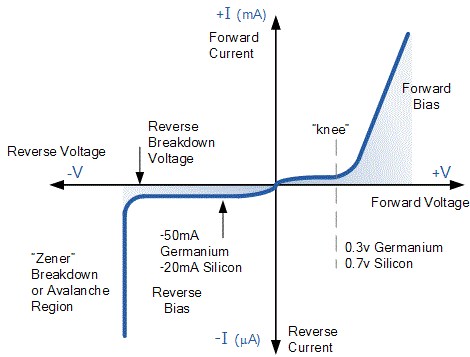
\includegraphics[width=0.4\textwidth]{zener.png}
	\caption{Typical Characteristics for a Zener Diode(Source: The Internet)}
\end{figure}
A Zener diode is a special type of diode that is designed to operate in reverse bias, unlike 
regular diodes which operate in forward bias. The Zener diode is designed to have a sharp 
increase in output current when the voltage across the diode reaches a threshold value called 
the breakdown voltage. The breakdown voltage is also called the Zener voltage.

When the diode is in reverse bias, there is a range where the current remains very small(in the 
$\mu A$ range), after which the current increases sharply. This is the breakdown region. Here the 
voltage across the Zener diode is regulated to be constant.

\begin{figure}[H]
    \centering
    % \begin{circuitikz}[american voltages]
    %     % Zener Diode with coloring
    %     \draw
    %     (5,-2) to [zzD, fill=cyan!40] (5,2)
    %     % Current meter and upper connections
    %     to [rmeter, t=mA, l_=$i_z$, fill=yellow!70] (5, 3)
    %     to [short, -*] (5, 4)
    %     to [rmeter, t=mA, l_=$i_s$, fill=yellow!70] (2, 4)
    %     to [R, l^=$R_s$] (1, 4)
    %     to [short] (0, 4)
    %     % Battery connection
    %     to [battery, l=$V_{\mathrm{in}}$] (0, -1)
    %     to [short] (0, -2)
    %     to [short] (5, -2)
    %     % Load branch
    %     (5, 4) to [short] (7, 4)
    %     to [R, l=$R_C$] (7, 2)
    %     to [rmeter, t=mA, l_=$i_L$, fill=yellow!70] (7, 1)
    %     to [vR, l=$R_{\mathrm{L}}$] (7, -2)
    %     to [short] (5, -2)
    %     % Probing points
    %     (7, 3.8) to [short, -*] (8.5, 3.8)
    %     (7, -1.5) to [short, -*] (8.5, -1.5);
    % \end{circuitikz}
   \resizebox{0.5\textwidth}{!}{\begin{tikzpicture}
	% Paths, nodes and wires:
	\draw (12.75, 3.202) to[variable american resistor, l={$R_L$}, label distance=0.02cm] (12.75, 0.952);
	\draw (5.5, 4.75) to[battery, l={$V_i(V)$}, label distance=0.02cm] (5.5, 4.5);
	\draw (5.5, 6.75) to[american resistor, l={$R_s$}, label distance=0.02cm] (7.75, 6.75);
	\draw (7.75, 6.75) to[ammeter, name=mA, l={$I_s (mA)$}, label distance=0.02cm] (9, 6.702);
	\draw (10.75, 6.202) to[ammeter, l_={$I_z(mA)$}, label distance=0.02cm] (10.712, 5.5);
	\draw (12.788, 3.904) to[ammeter, l_={$I_L(mA)$}, label distance=0.02cm] (12.75, 3.202);
	\draw (10.712, 5.5) -| (10.75, 3.5);
	\draw (9, 6.702) -| (10.75, 6.202) -| (10.75, 6.702) -| (12.75, 6.202);
	\draw (12.75, 6.202) to[american resistor, l={$R_c$}, label distance=0.02cm] (12.75, 3.952);
	\draw (5.5, 6.75) -| (5.5, 4.75);
	\draw (5.5, 4.5) |- (12.75, 0.952);
	\draw (10.75, 0.952) to[full ZZener diode, l={$D_z$}, label distance=0.02cm] (10.75, 3.5);
	\draw (15, 6.25) to[voltmeter, l={$V_o(V)$}, label distance=0.02cm] (15, 1.25);
	\draw (12.75, 6.202) |- (15, 6.25);
	\draw (12.75, 1.25) -- (15, 1.25);
\end{tikzpicture}}
    \caption{Circuit Diagram for Load and Line Regulation Using a Zener Diode}
\end{figure}
From the cicuit diagram above, we get the following equations finding out the voltages at the nodes.
\begin{align}
	I_s = I_z + I_L \\ 
	I_s = \frac{V_i - V_z}{R_s} \\
	I_L = \frac{V_o}{R_c+R_L}
\end{align}
For our first line regulation experiment with the zener diode $R_L = 0, R_s = 2.2k\Omega, R_c = 2.2k\Omega$.
Here, when we operate in the breakdown region , $V_o$ is kept constant and $V_i$ is varied. From here 
we get that 
\begin{align}
	\delta I_s = \delta I_z
\end{align}
So ignoring the initial points, we should get a linear relation between $I_z$ and $I_s$ with slope 1, in the
breakdown region. The Voltage does saturate and gets regulated in the breakdown region, but
increase slowly and linearly with $V_i$.

For the load regulation experiment, we keep $V_i$ constant and vary $R_L$. Here, we get that
\begin{align}
	\delta I_z = -\delta I_L
\end{align}
So, we should get a linear relation between $I_z$ and $I_L$ in the breakdown region with 
a slope of $-1$. The voltage remains constant with the change in $R_L$ as well.
\subsection{IC 7805}
Using the Zener Diode, the voltage regulation is not perfectly constant, and increases 
slowly and linearly with $V_i$. The IC 7805 is a voltage regulator that is much more efficient
 and much better at voltage regulation than a Zener Diode. The IC 7805 is a 3-terminal device 
 with an input, ouput and a ground pin. The IC 7805, as the name suggests,
 regulates the output voltage to be 5V. The input pin of the of the IC 7805 is connected to the
 Input source Voltage and the output is connected the node where the output voltage is to be measured.
\begin{figure}[H]
    \centering
    \resizebox{0.5\textwidth}{!}{
        \begin{tikzpicture}
	% Paths, nodes and wires:
	\draw (12.75, 3.202) to[variable american resistor, l={$R_L$}, label distance=0.02cm] (12.75, 0.952);
	\draw (5.5, 4.75) to[battery, l={$V_i(V)$}, label distance=0.02cm] (5.5, 4.5);
	\draw (12.788, 3.904) to[ammeter, l_={$I_L(mA)$}, label distance=0.02cm] (12.75, 3.202);
	\draw (12.75, 6.202) to[american resistor, l={$R_c$}, label distance=0.02cm] (12.75, 3.952);
	\draw (5.5, 6.75) -| (5.5, 4.75);
	\draw (5.5, 4.5) |- (12.75, 0.952);
	\draw (15, 5.798) to[voltmeter, l={$V_o(V)$}, label distance=0.02cm] (15, 1.25);
	\draw (12.75, 5.75) |- (15, 5.798);
	\draw (12.75, 1.25) -- (15, 1.25);
	\node[shape=rectangle, draw, line width=1pt, inner sep=0, minimum width=0.965cm, minimum height=0.965cm](Rect1) at (9.5, 8){} node[anchor=south] at (Rect1.north){$IC  7805$};
	\draw (9.25, 7.5) |- (5.5, 6.75);
	\draw (9.5, 7.5) -- (9.5, 1);
	\draw (12.75, 6.202) -| (9.75, 7.5);
\end{tikzpicture}
    }
    \caption{Circuit Diagram for Load and Line Regulation Using a IC 7805}
\end{figure}
\section{Zener Diode}
\subsection{Line Regulation}
The data for the Line regulation using a Zener Diode is given here in Table \ref{tab:ZD linereg} in the Supplementary Section.
We fix $R_s=R_c =2.2 k\Omega$ and $R_L = 0 k\Omega$ and varied the input voltage. The data is plotted in the following figures.
We obtain a linear fit between $I_z$ and $I_s$ with slope $\pmb{1.002 \pm 0.016}$, which matches our theoretical predictions.
The graph between the input and output voltage is also plotted. \\

From the data, we can see that the output voltage corresponding to $V_{min} = 10.51 V$. 
The output voltage reaches almost saturation near
the input voltage of $V_{min}=10.51V$, which gives us a breakdown voltage of \\
\begin{center}\fbox{$V_b = 4.34V$}\end{center}

\begin{figure}[H]
	\centering
	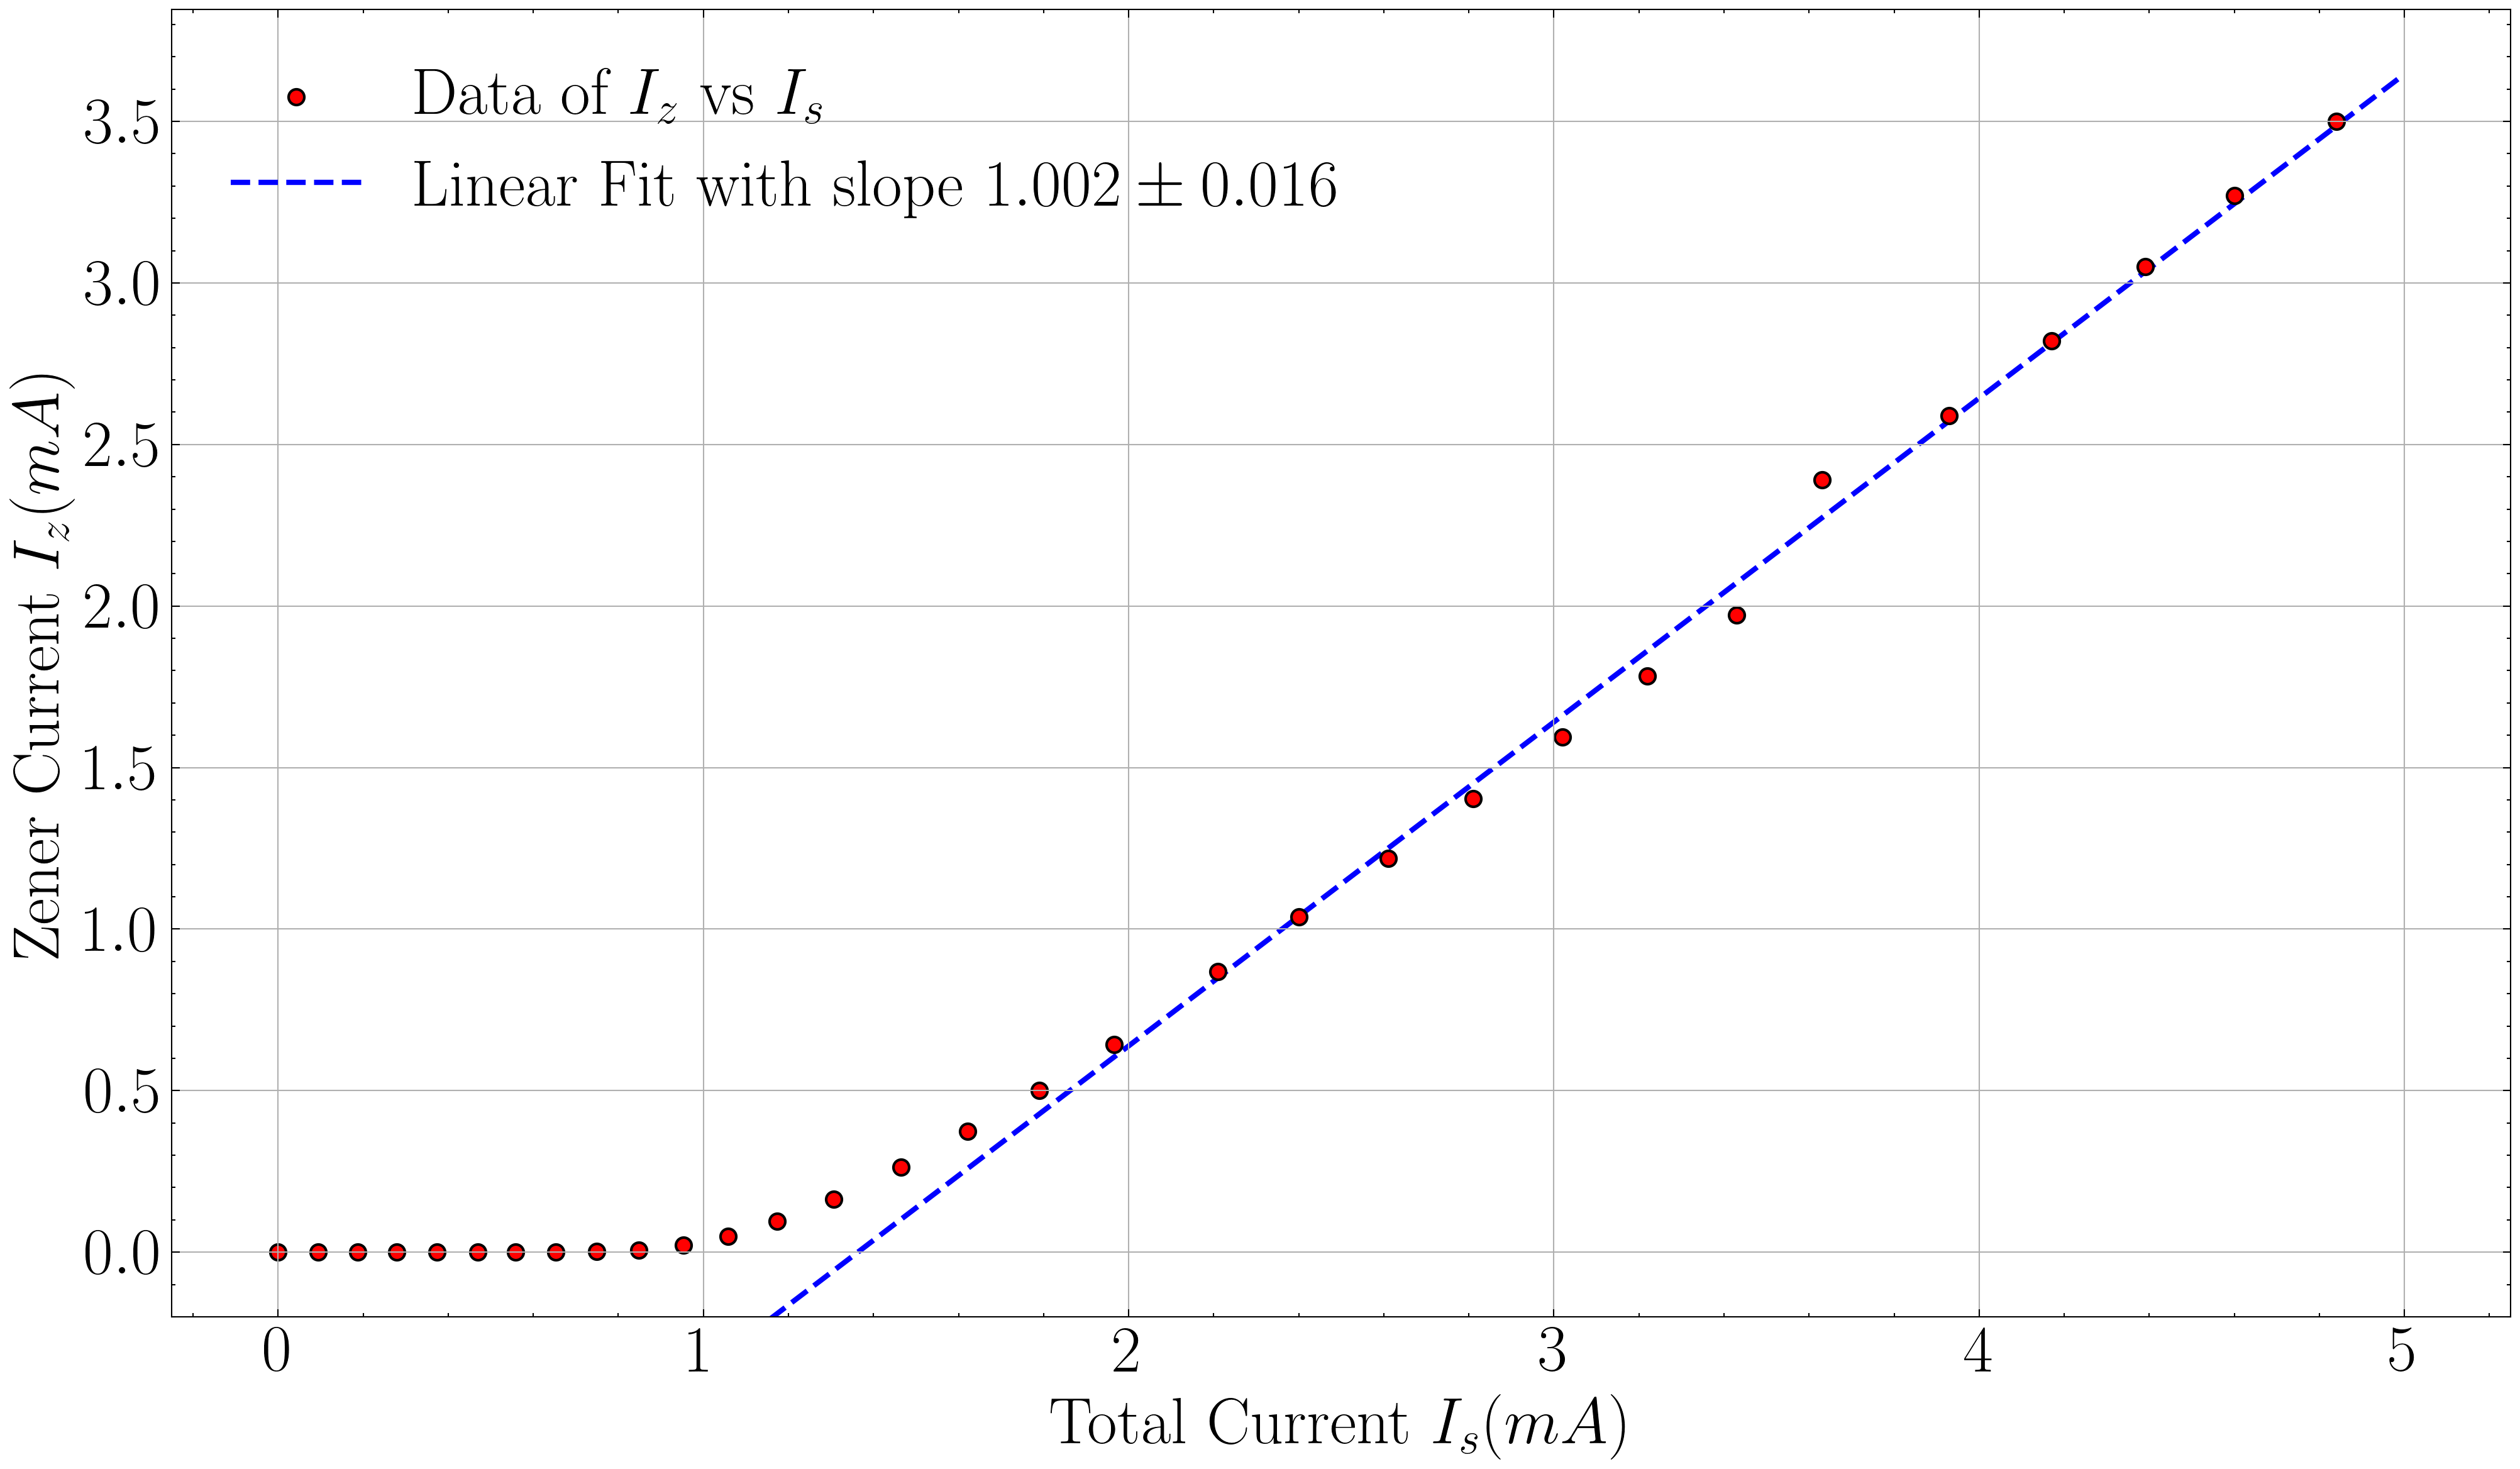
\includegraphics[width=0.8\textwidth]{zlinereg_iz_is.png}
	\caption{$I_z$ vs $I_s$ for Zener Diode Line Regulation}
\end{figure}
\begin{figure}[H]
	\centering
	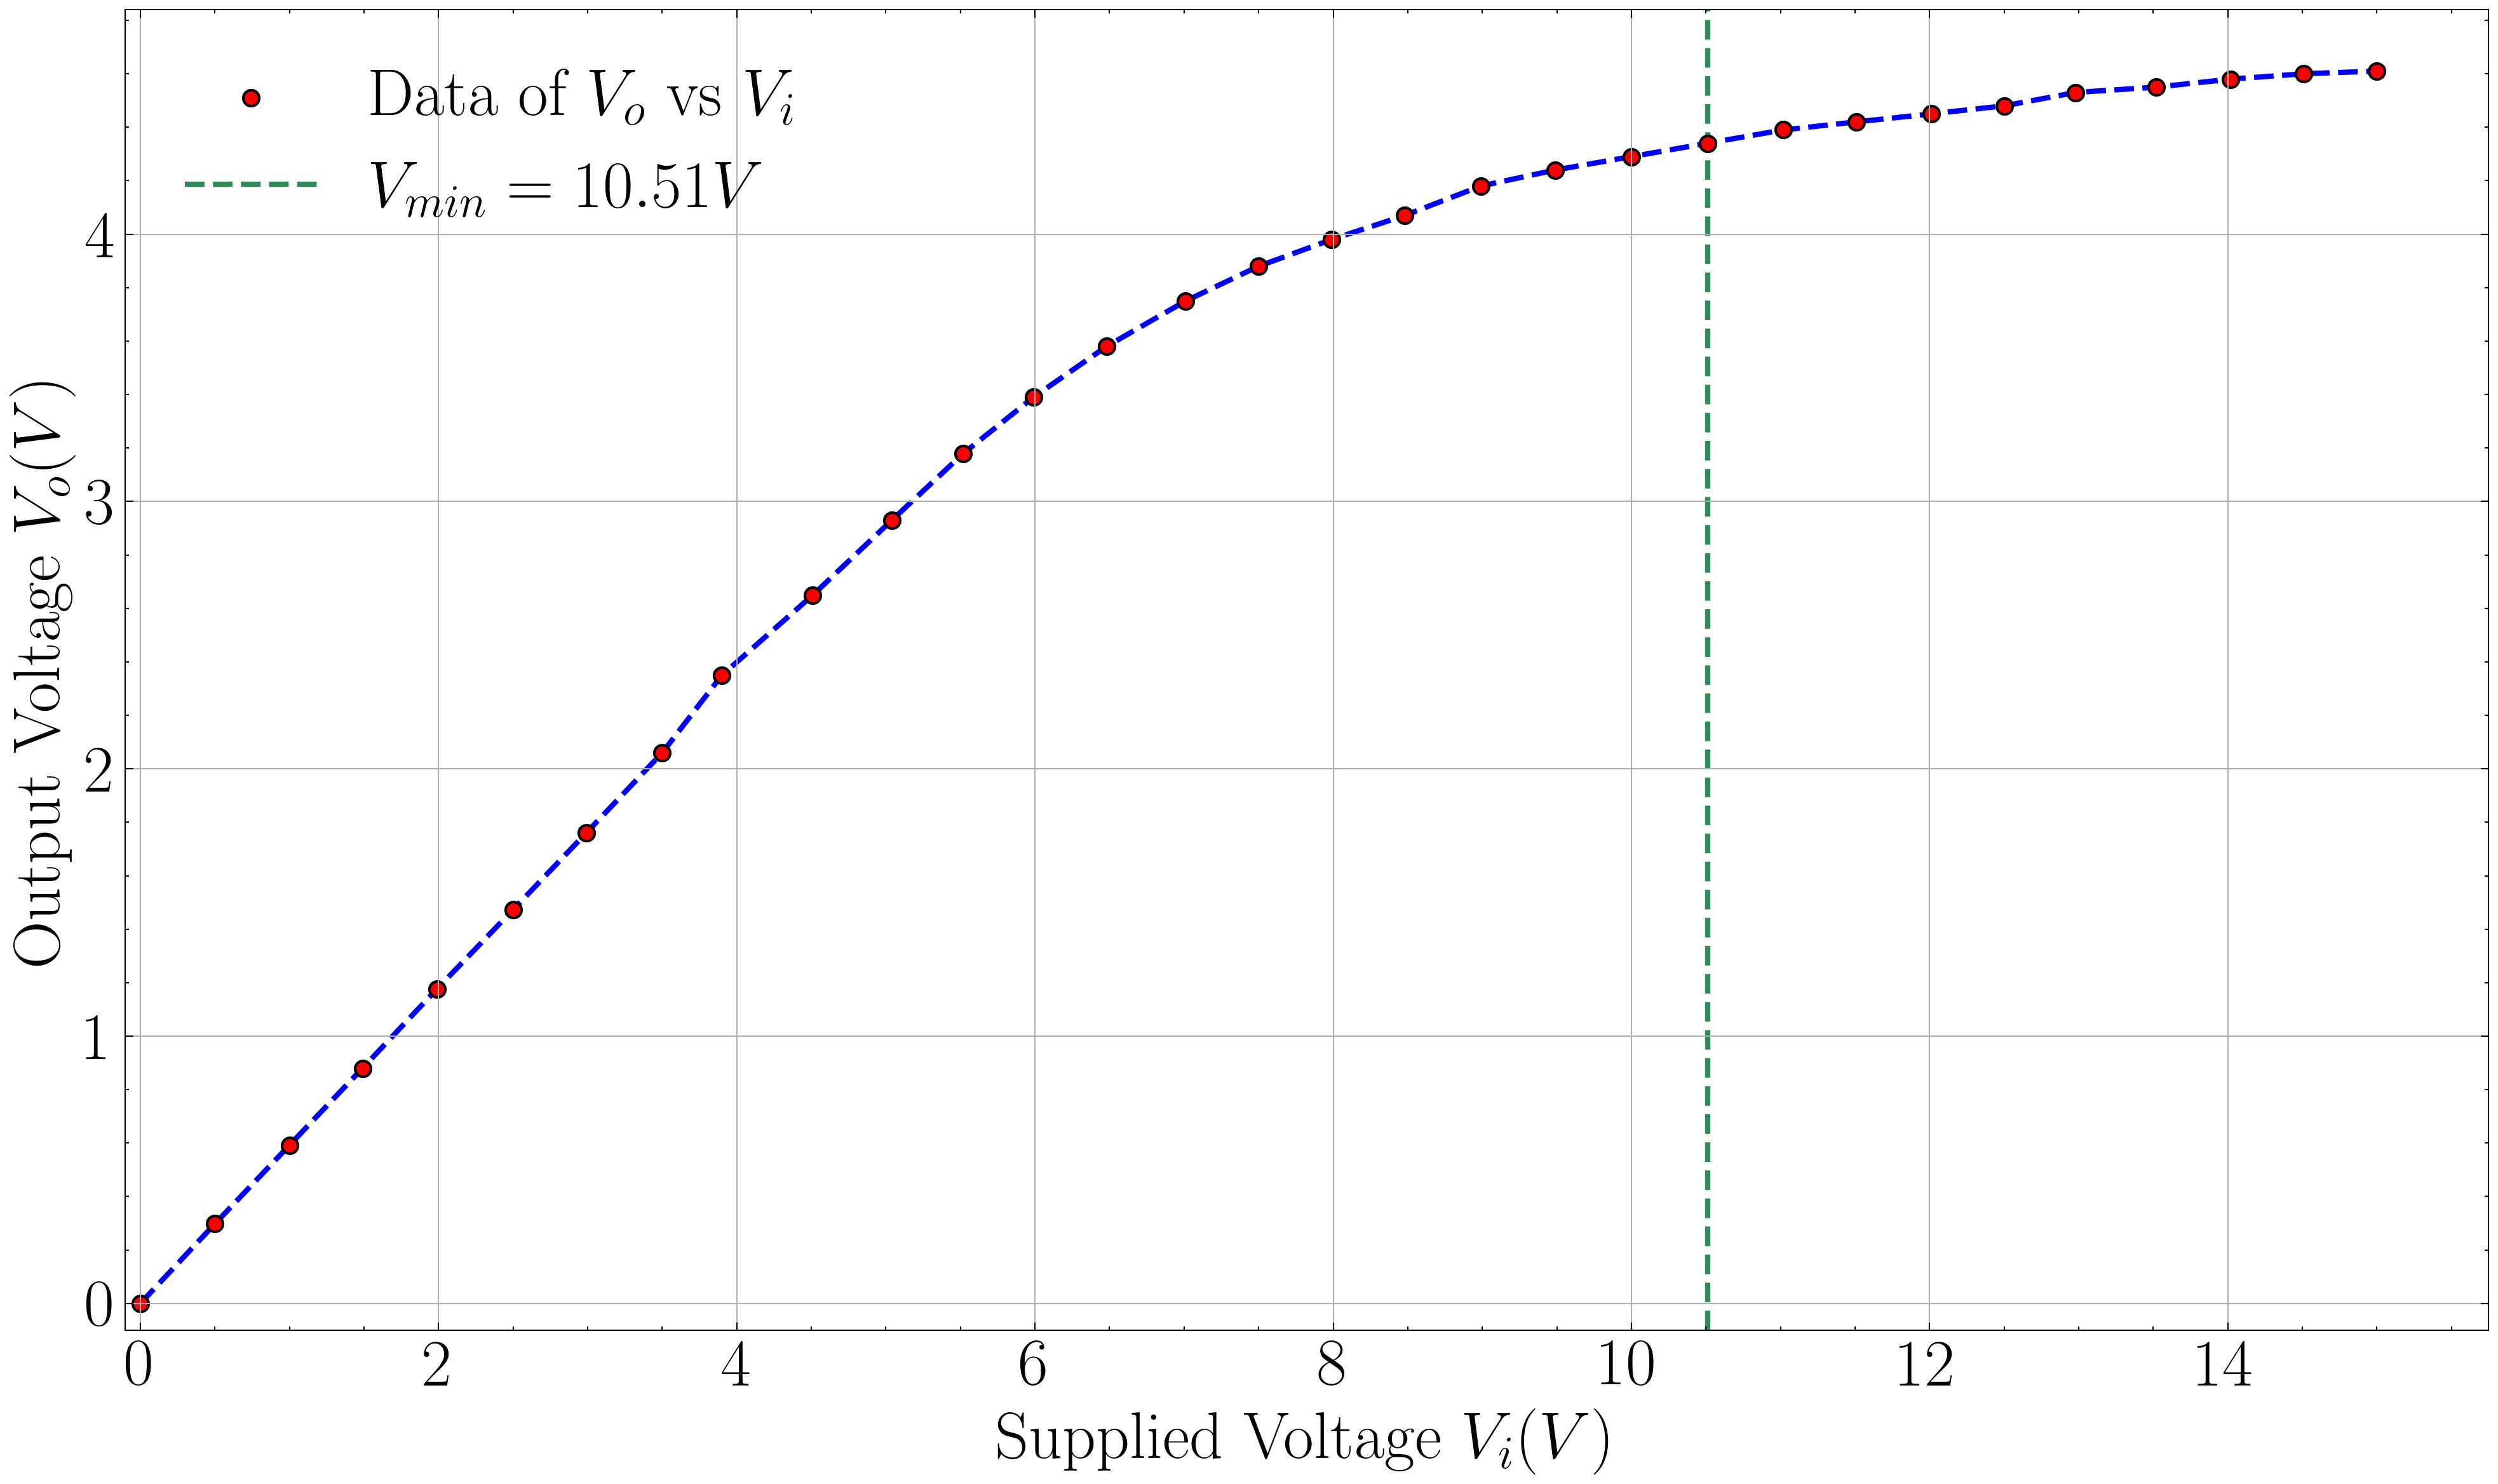
\includegraphics[width=0.8\textwidth]{zlinereg_vo_vi.png}
	\caption{$V_o$ vs $V_i$ plot for  Zener Diode Line Regulation}
\end{figure}
\subsection{Load Regulation}


\subsubsection{Approaching Breakdown Region}
The aim of this part was to see the approach to the breakdown voltage using some value of 
$R_c$ that doesnt push the Zener to its breakdown region. To find out this value, we used to two potentiometers
one acting as $R_c$ and the other acting as $R_L$. We varied the value of $R_c$ and $R_L$ to see the approach to the breakdown region.
We then fixed the value of $R_c=1k\Omega$ and varied the value of $R_L$ to see the load regulation. The data is given in Table \ref{tab:ZDload1ohm} in the Supplementary Section.

\textbf{Note:} This experiment was done on Day 2 on which we received a different Zener diode with a different
breakdown voltage. The breakdown voltage was found to be around $V_b = 6.44V$, which is different from the breakdown voltage of 
the previous Zener Diode, used for line regulation and load regulation in the breakdown region, where $V_b \approx 4.5 V$.
\begin{figure}[H]
	\centering
	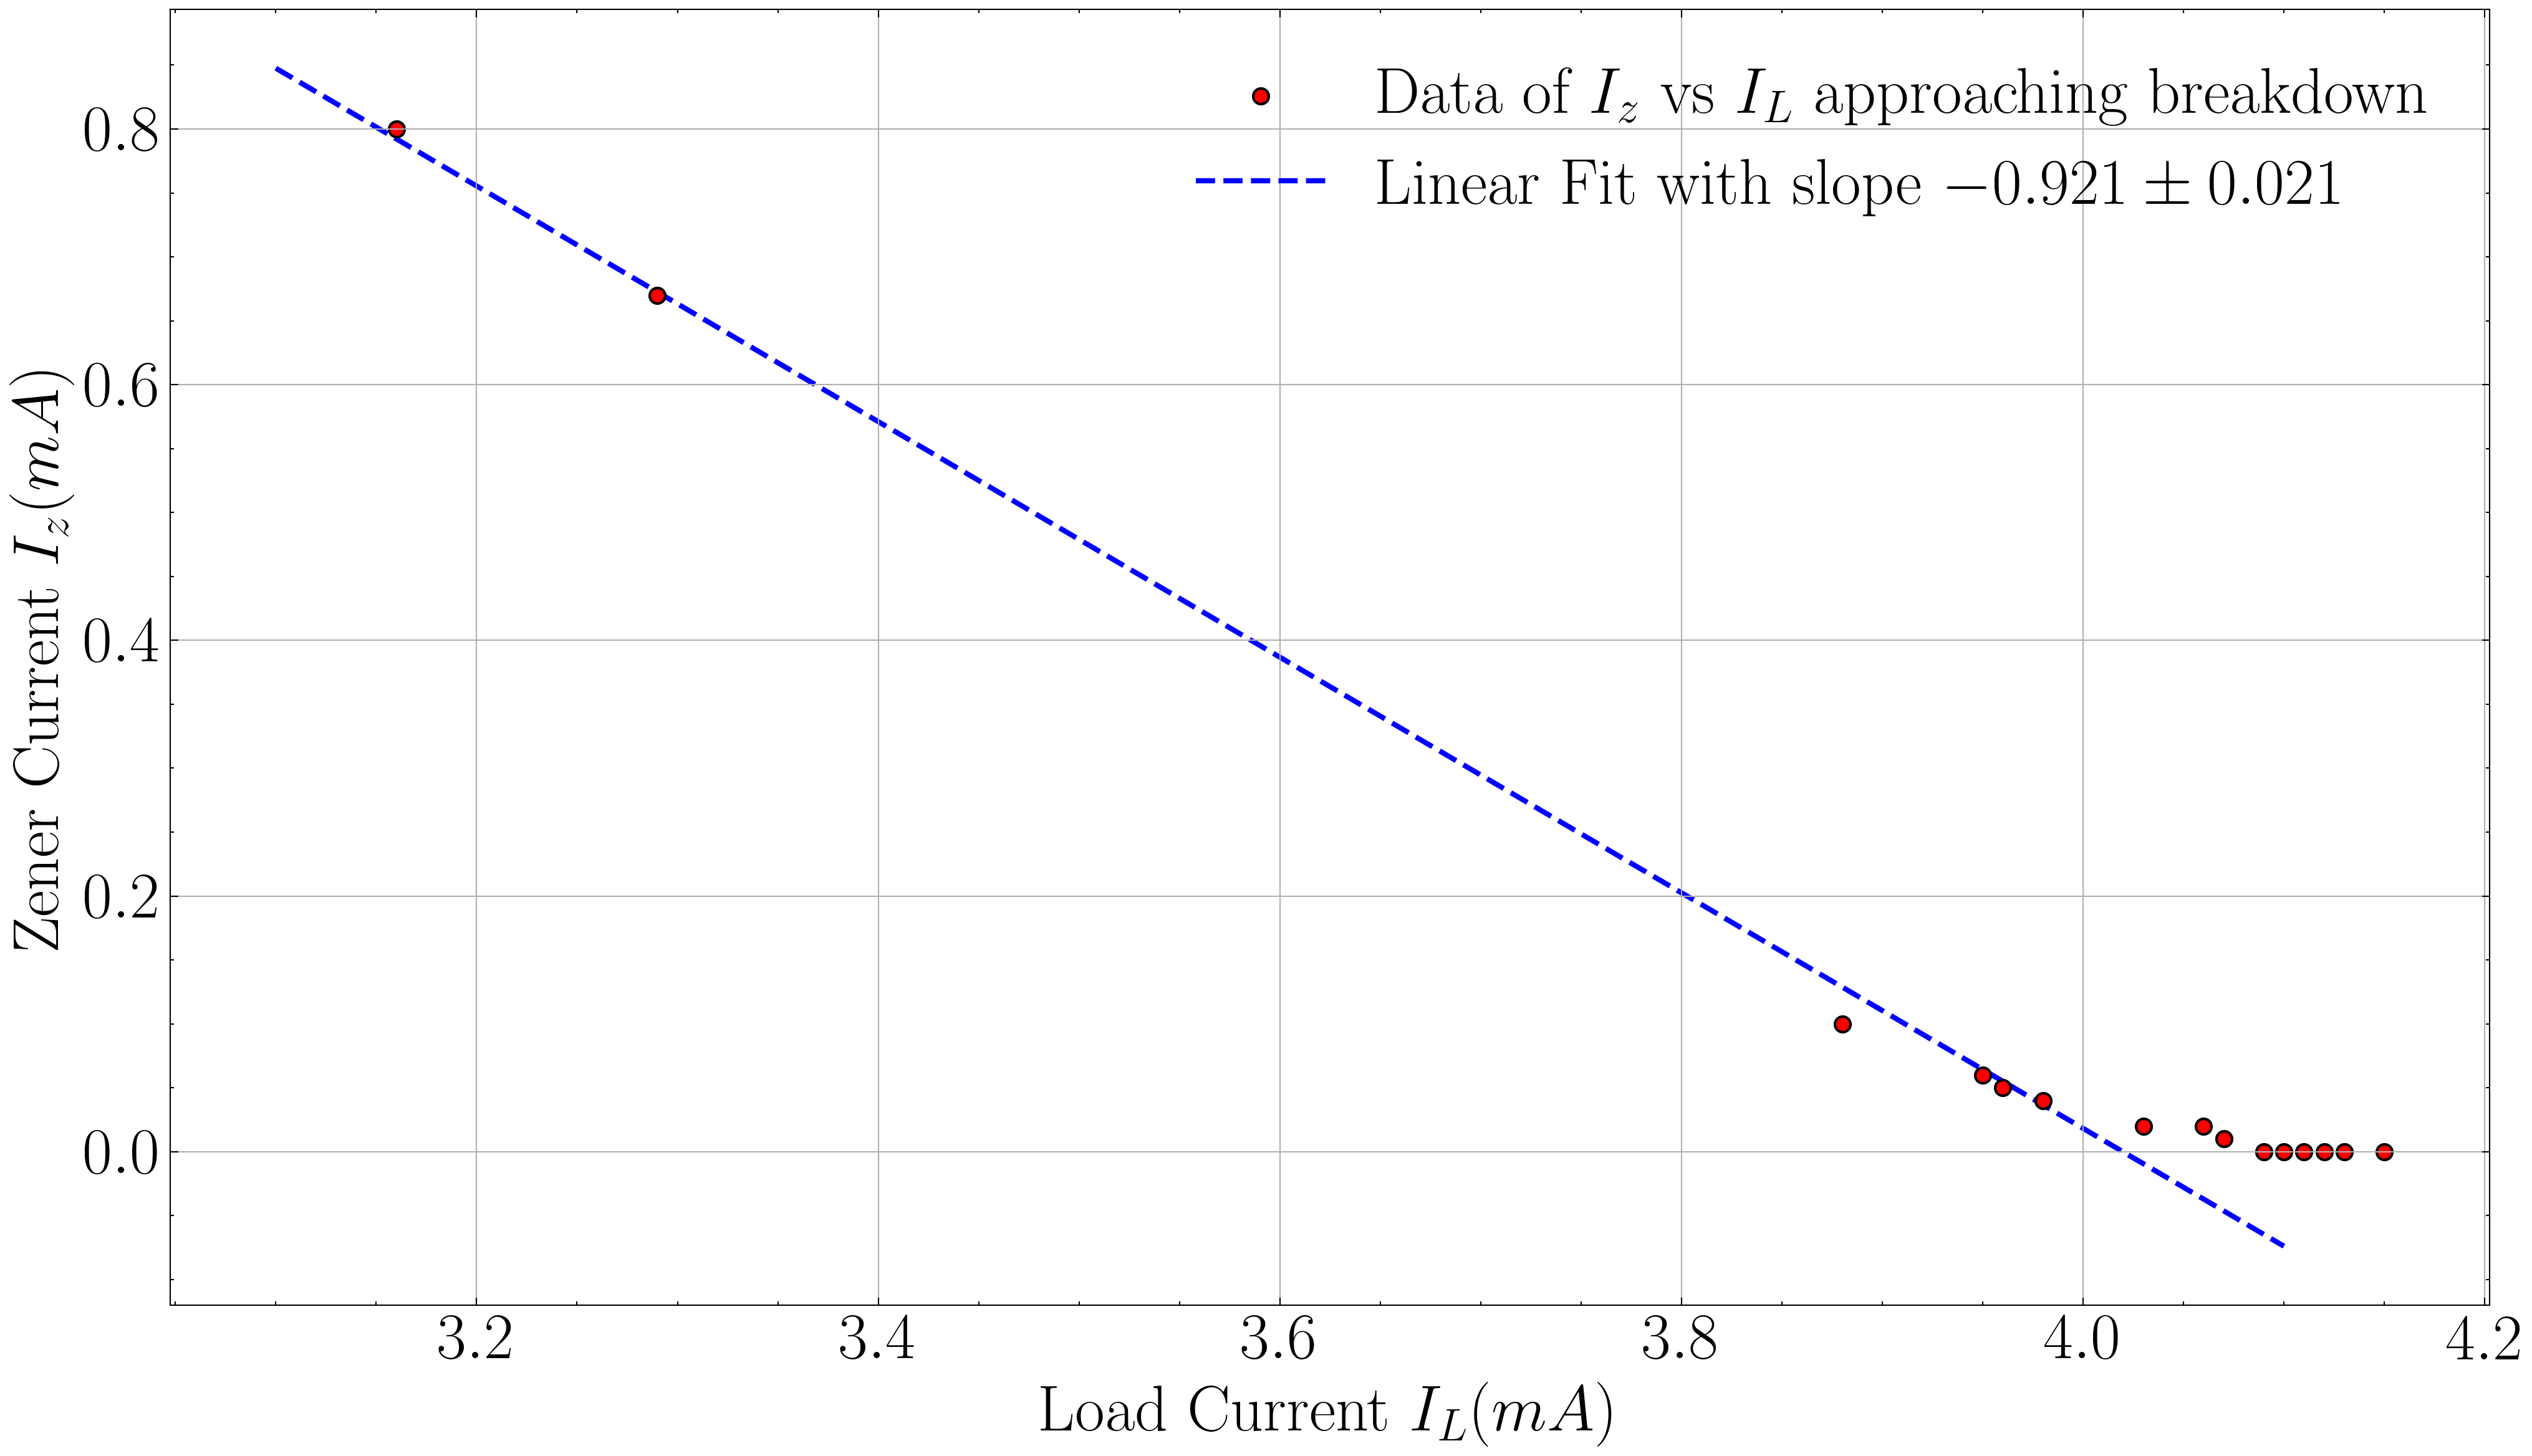
\includegraphics[width=0.8\textwidth]{zloadreg_iz_il.png}
	\caption{$I_z$ vs $I_L$ plot for Zener Diode Load Regulation}
\end{figure}
\begin{figure}[H]
	\centering
	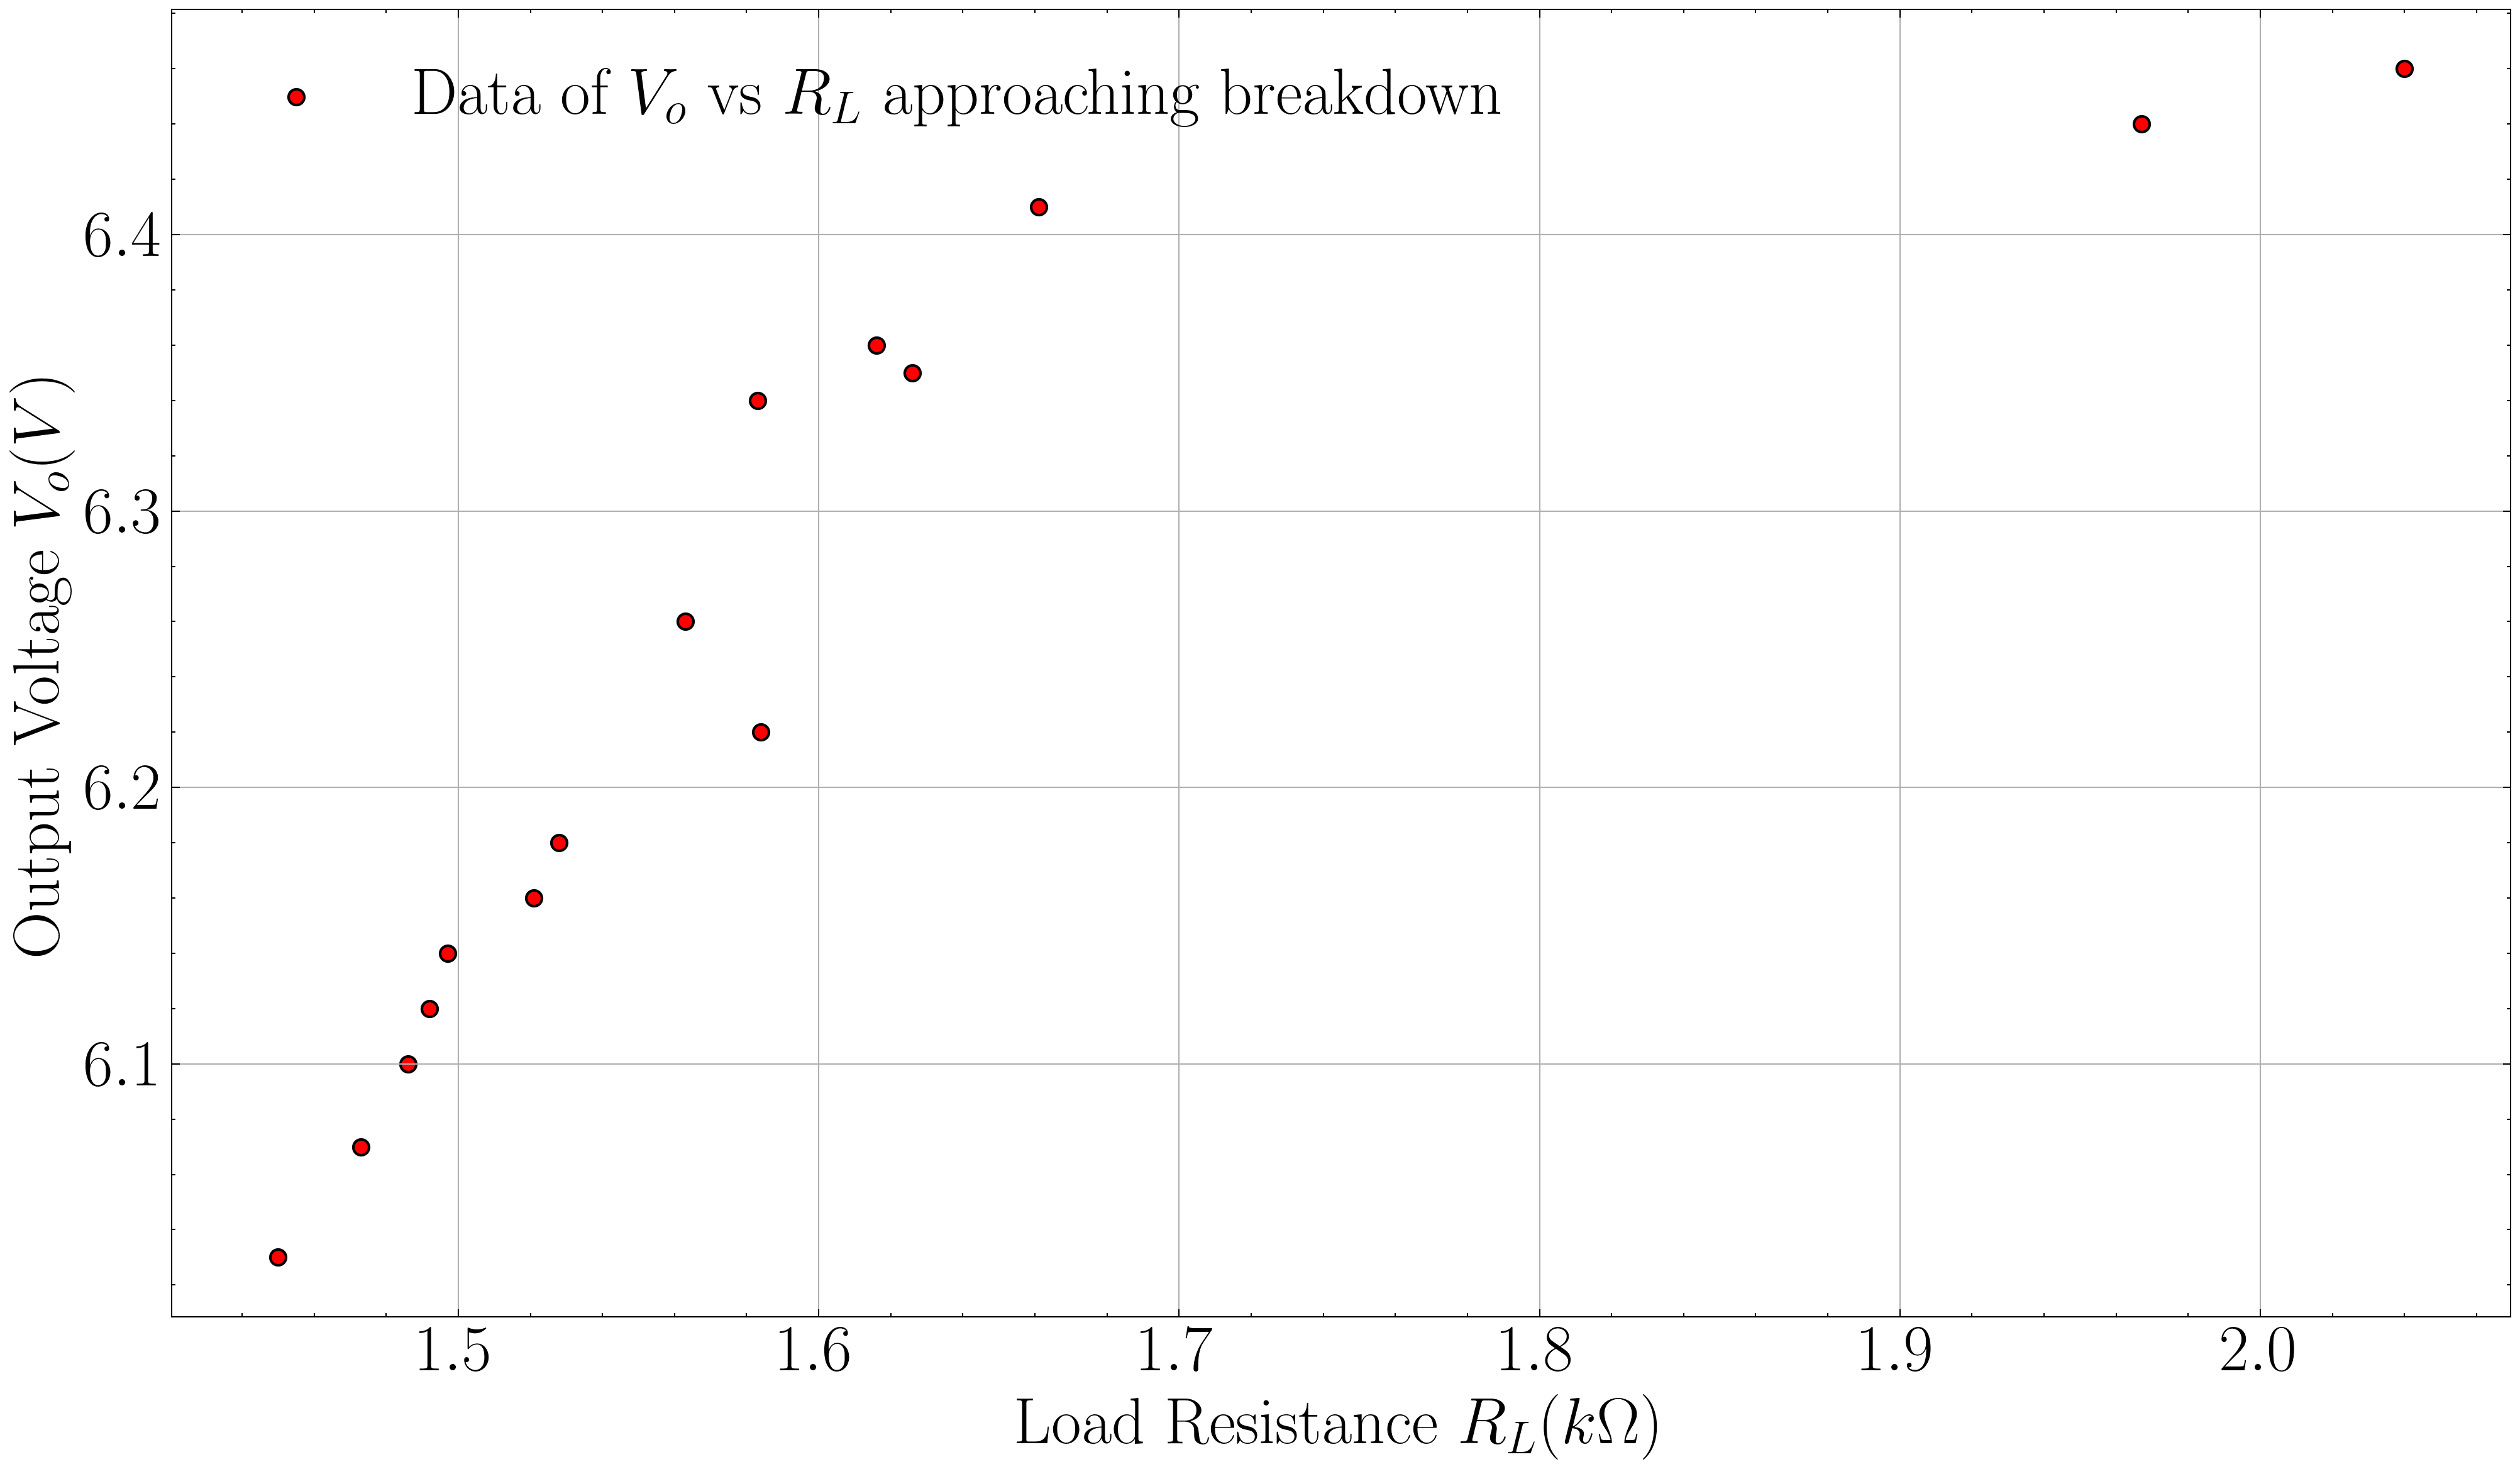
\includegraphics[width=0.8\textwidth]{zloadreg_vo_rl.png}
	\caption{$V_o$ vs $R_L$ plot for Zener Diode Load Regulation}
\end{figure}
In the later part in the approach to the breakdown region, we get a linear relation between $I_z$ and $I_L$ with a slope of $\pmb{-0.921 \pm 0.021}$, which 
verifies $\delta I_z = - \delta I_L$. 


The breakdown Voltage $V_b$ is found out to be \\ 

\begin{center}\fbox{$V_b = 6.44V$}\end{center}
\subsubsection{With Rc}
Here, for this experiment an $R_c = 2.2 k\Omega$ is added so that the Zener Diode is pushed to its breakdown region. 
The data is given in Table \ref{tab:ZDload2.2ohm} in the Supplementary Section. 


Here again, we expect $\delta I_z = -\delta I_L$ and we get a linear relation between $I_z$ and $I_L$ with a slope of $\pmb{-0.96 \pm 0.019}$, which
verifies out theoretical predictions. 

The breakdown voltage is the average voltage over which the whole experiment takes place since,
the Zener is already in its breakdown region. The breakdown voltage is found to be \\
\begin{center}\fbox{$V_b = (4.59 \pm 0.016)V$}\end{center}
\begin{figure}[H]
	\centering
	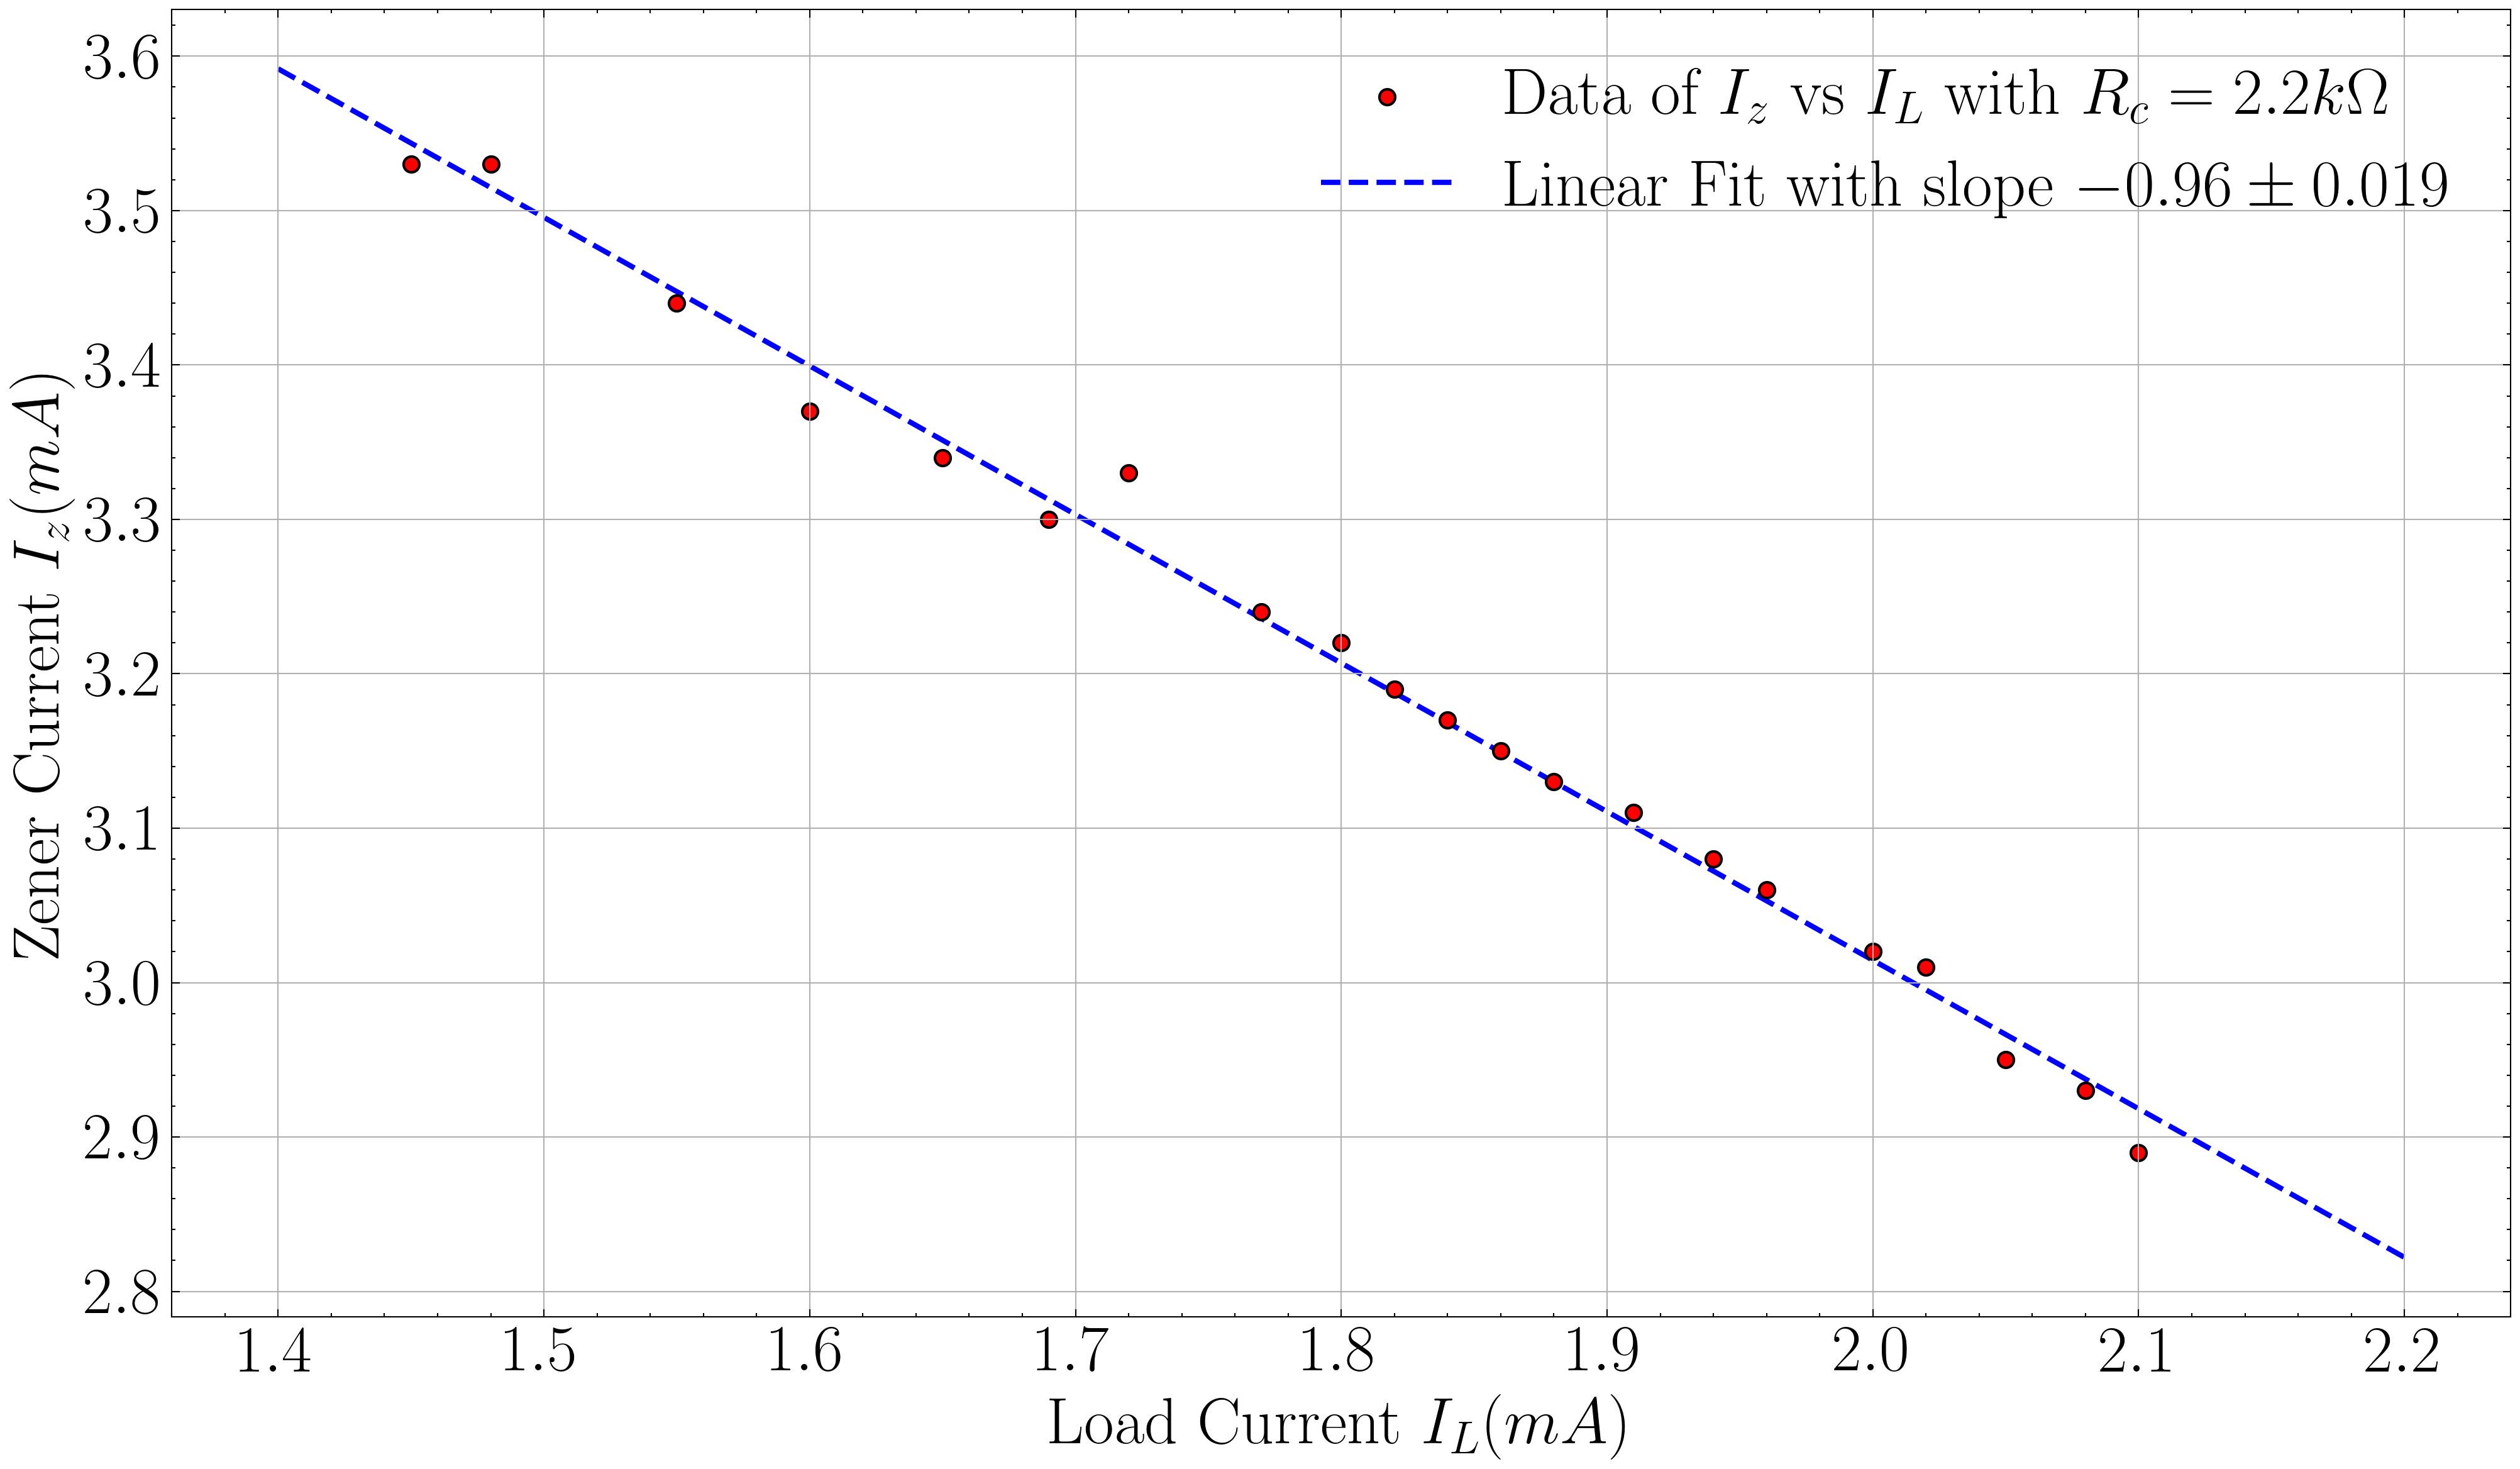
\includegraphics[width=0.8\textwidth]{zloadreg_iz_il_rc.png}
	\caption{$I_z$ vs $I_L$ plot for Zener Diode Load Regulation with $R_c = 2.2 k\Omega$}
\end{figure}
\begin{figure}[H]
	\centering
	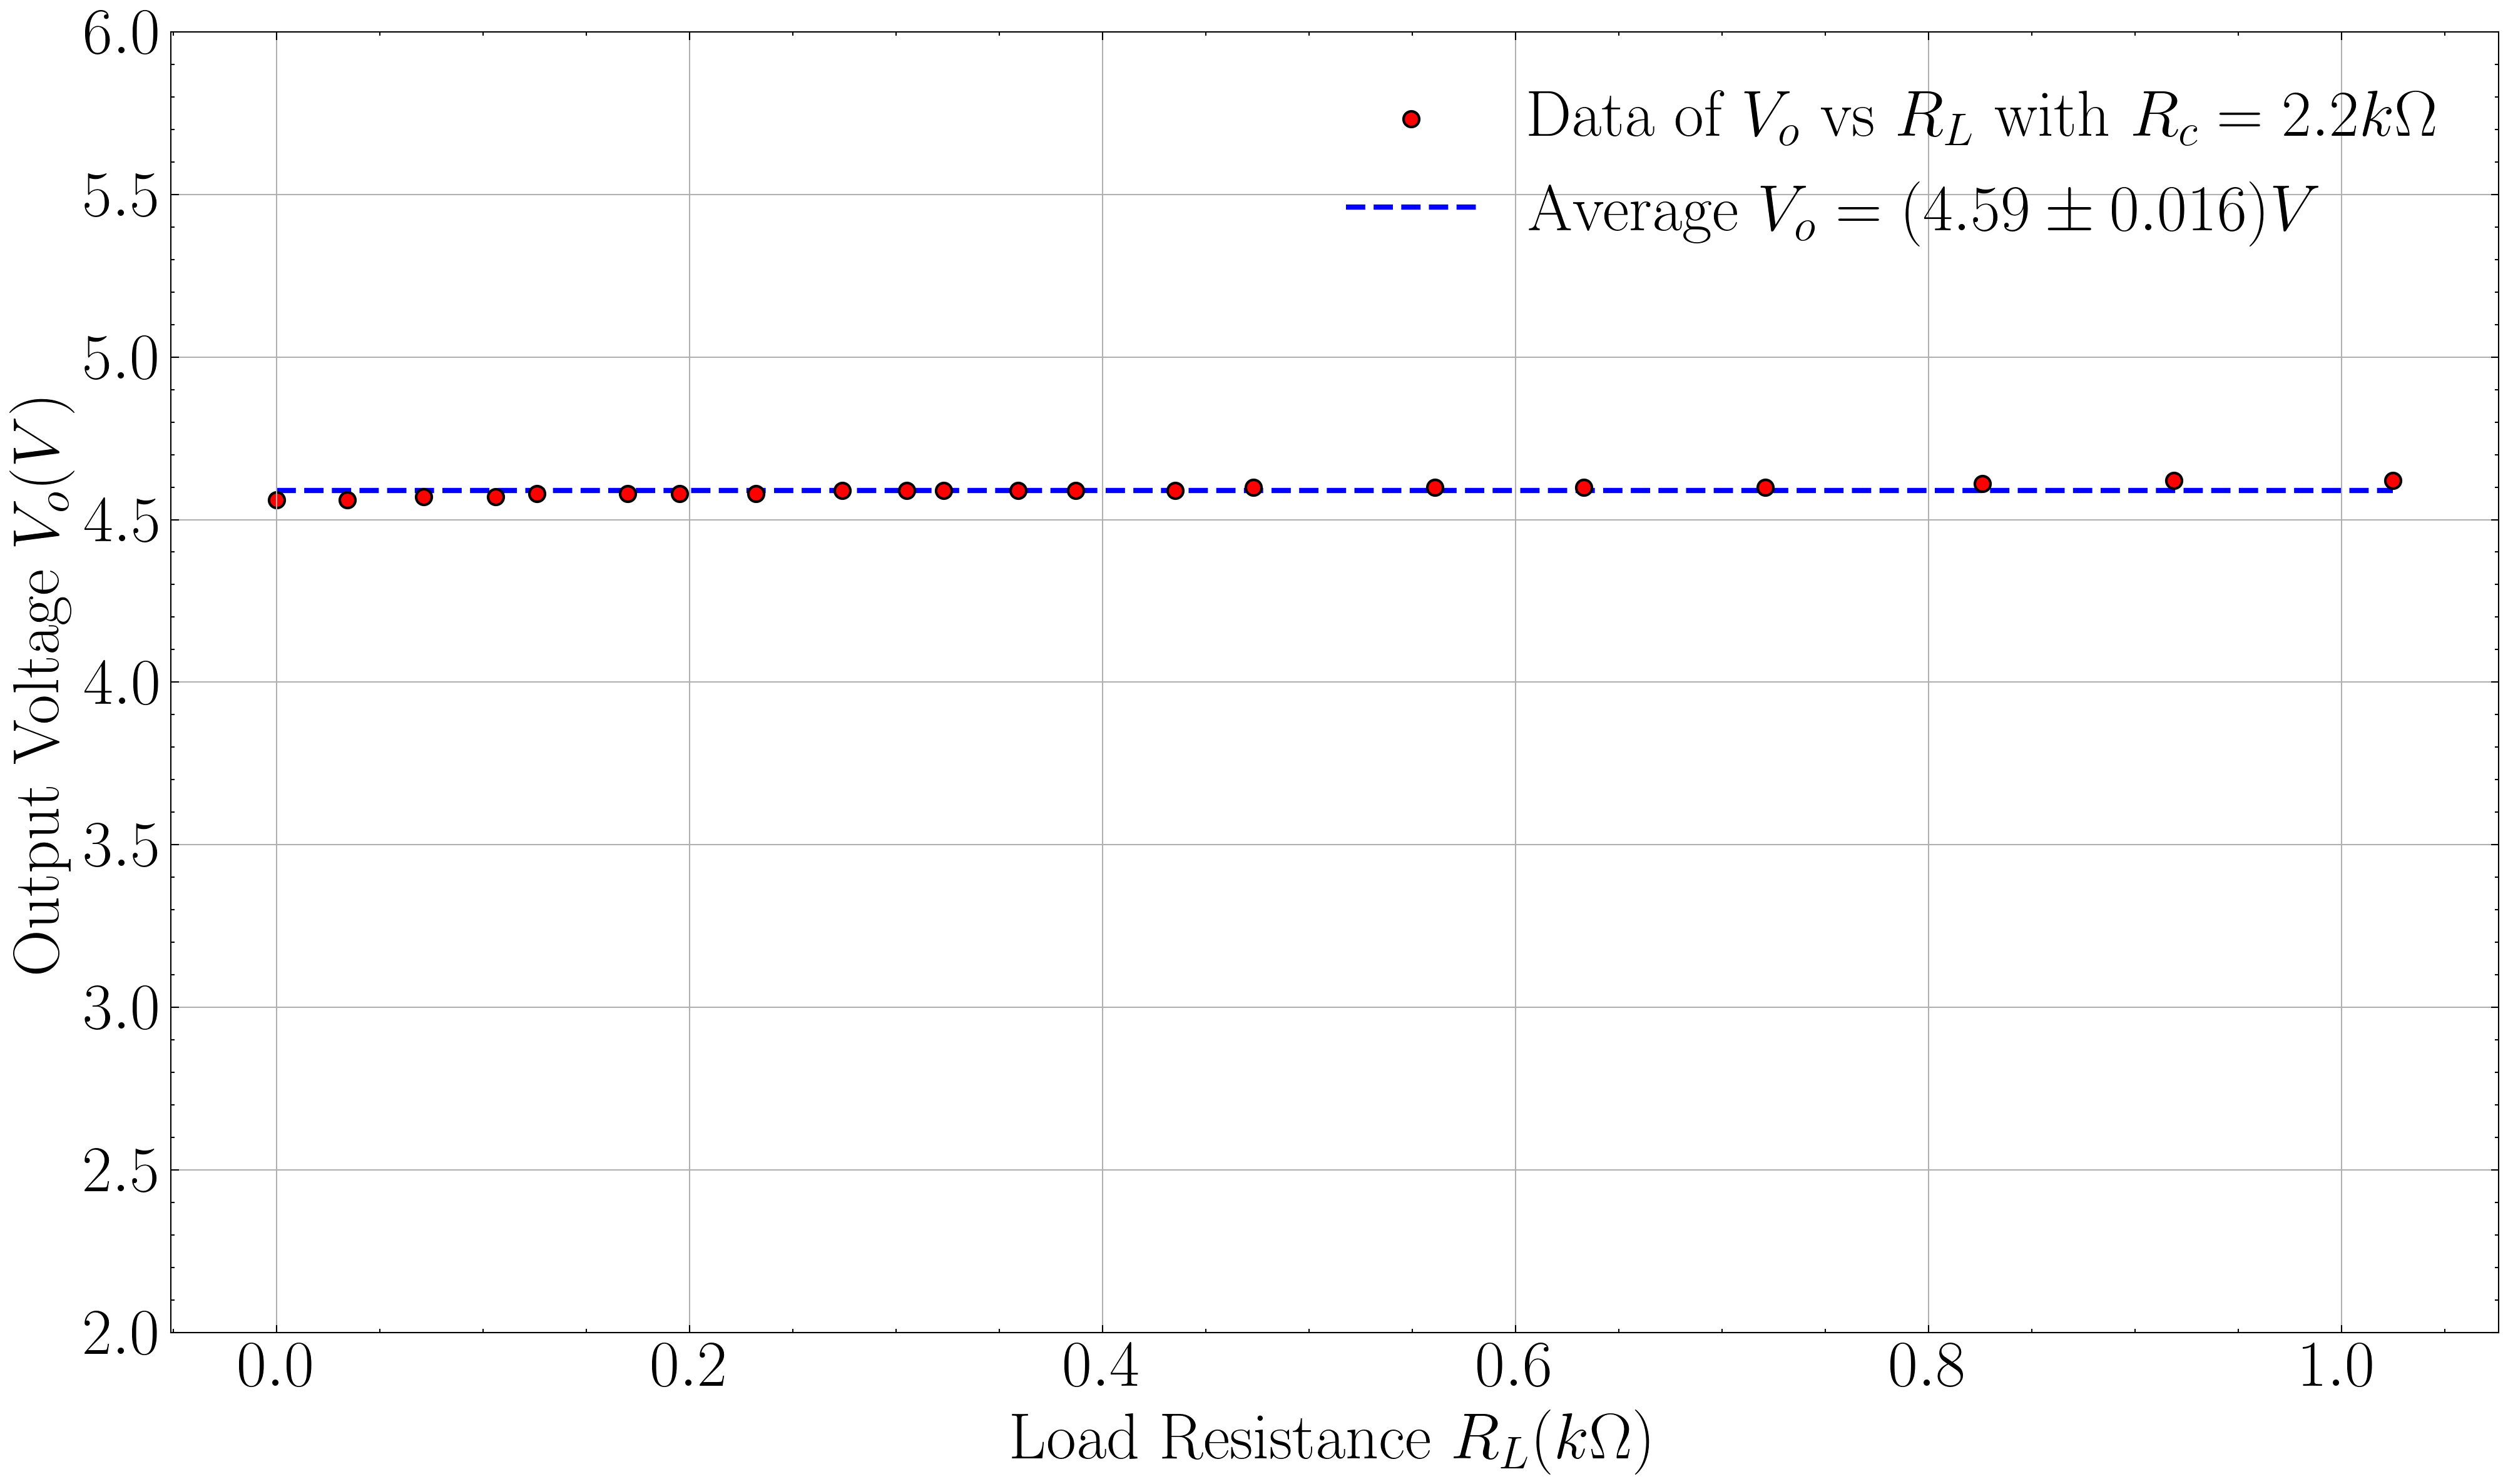
\includegraphics[width=0.8\textwidth]{zloadreg_vo_rl_rc.png}
	\caption{$V_o$ vs $R_L$ plot for Zener Diode Load Regulation with $R_c = 2.2 k\Omega$}
\end{figure}
\section{IC 7805}
\subsection{Line Regulation}
The data for the Line regulation using an IC 7805 is given here in Table \ref{tab:icline} in the Supplementary Section.
The voltage regulation in the breakdown region for the Zener Diode is not quite constant, so we use an IC here. 
From the graph, it is inferred that that the input voltage reaches $V_{clamp} = 6.48$ which gives our 
regulated Voltage $V_R$ as 
\begin{center}\fbox{$V_R = 5.11V$}\end{center}
The data shows that the clamping is quite efficient. It maintains the output voltage $V_o$ to 
be constantly at $V_R=5.11V$ upto the order of $10^{-2} V$, which is the resolution of our multimeter. 
\begin{figure}[H]
	\centering
	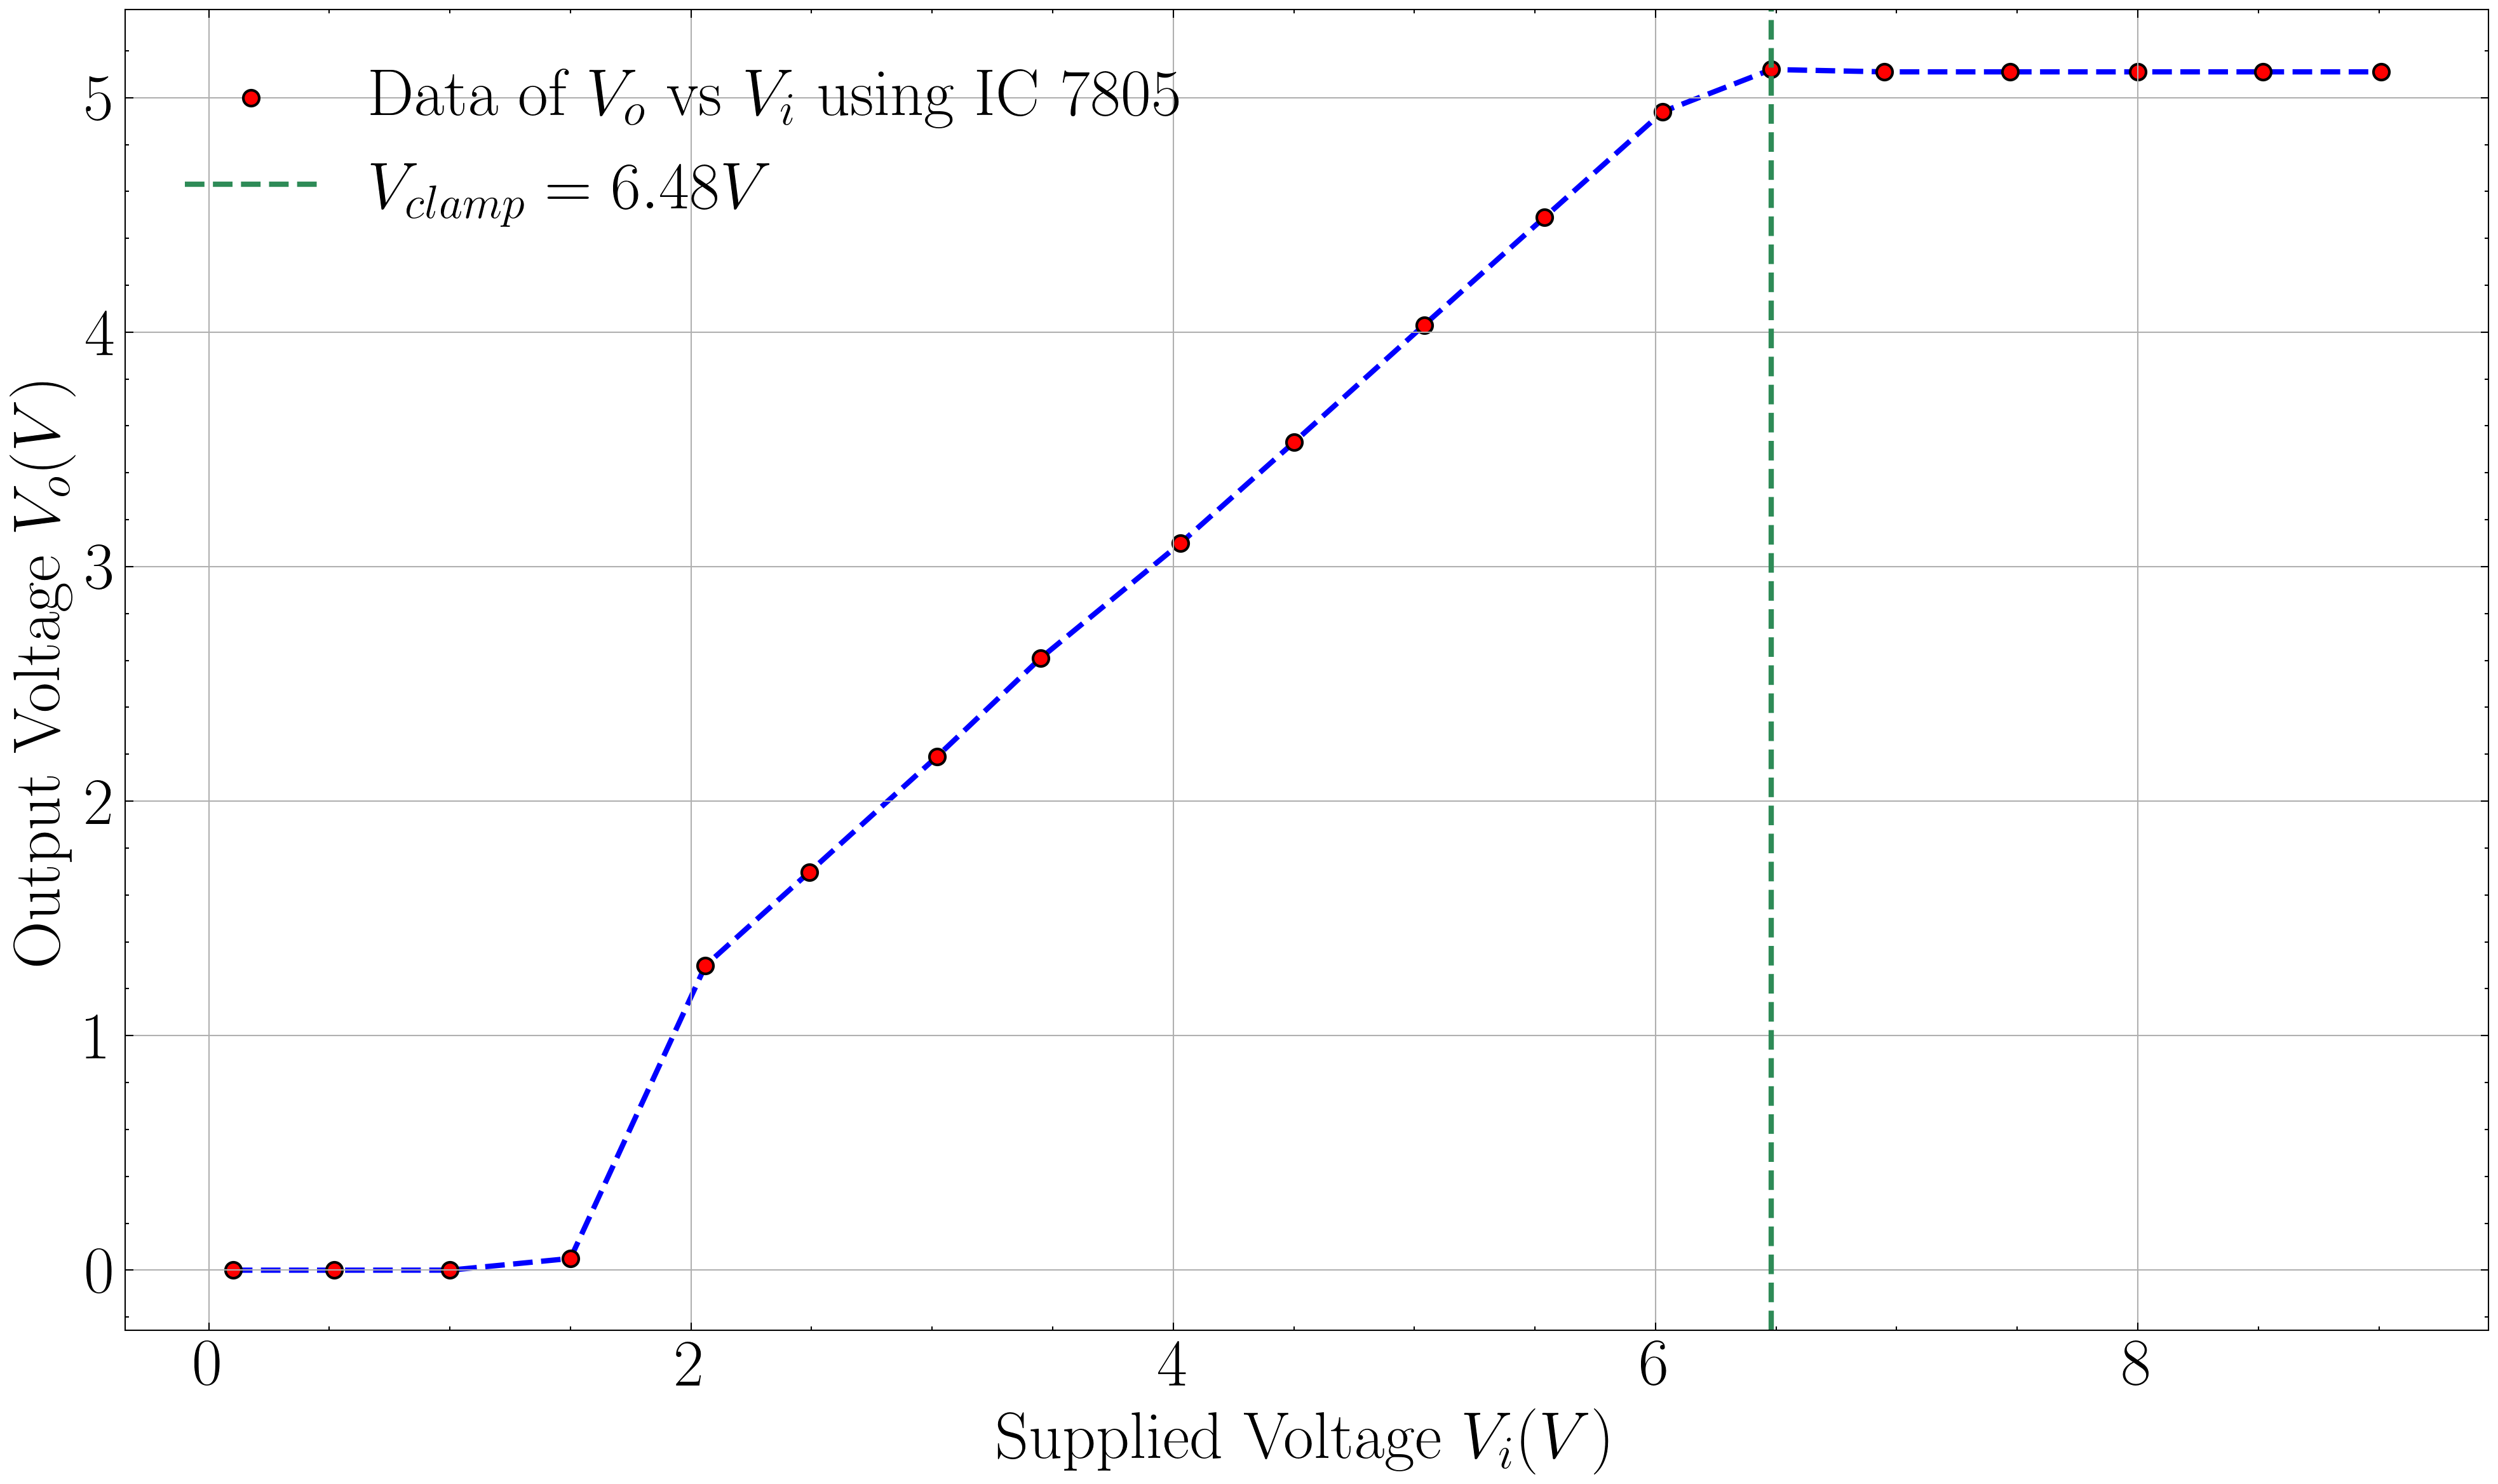
\includegraphics[width=0.8\textwidth]{iclinereg_vo_vi.png}
	\caption{$I_L$ vs $V_i$ plot for IC 7805 Line Regulation}
\end{figure}

\subsection{Load Regulation}
The data for Load regulation using the IC 7805 is given in Table \ref{tab:icload} in the Supplementary Section.
For load regulation, we vary over $R_L$ at the regulation voltage which is the average over the measured 
output voltages $V_R$,
\begin{center}\fbox{$V_R = (5.022 \pm 0.012)V$}\end{center}
\begin{figure}[H]
	\centering
	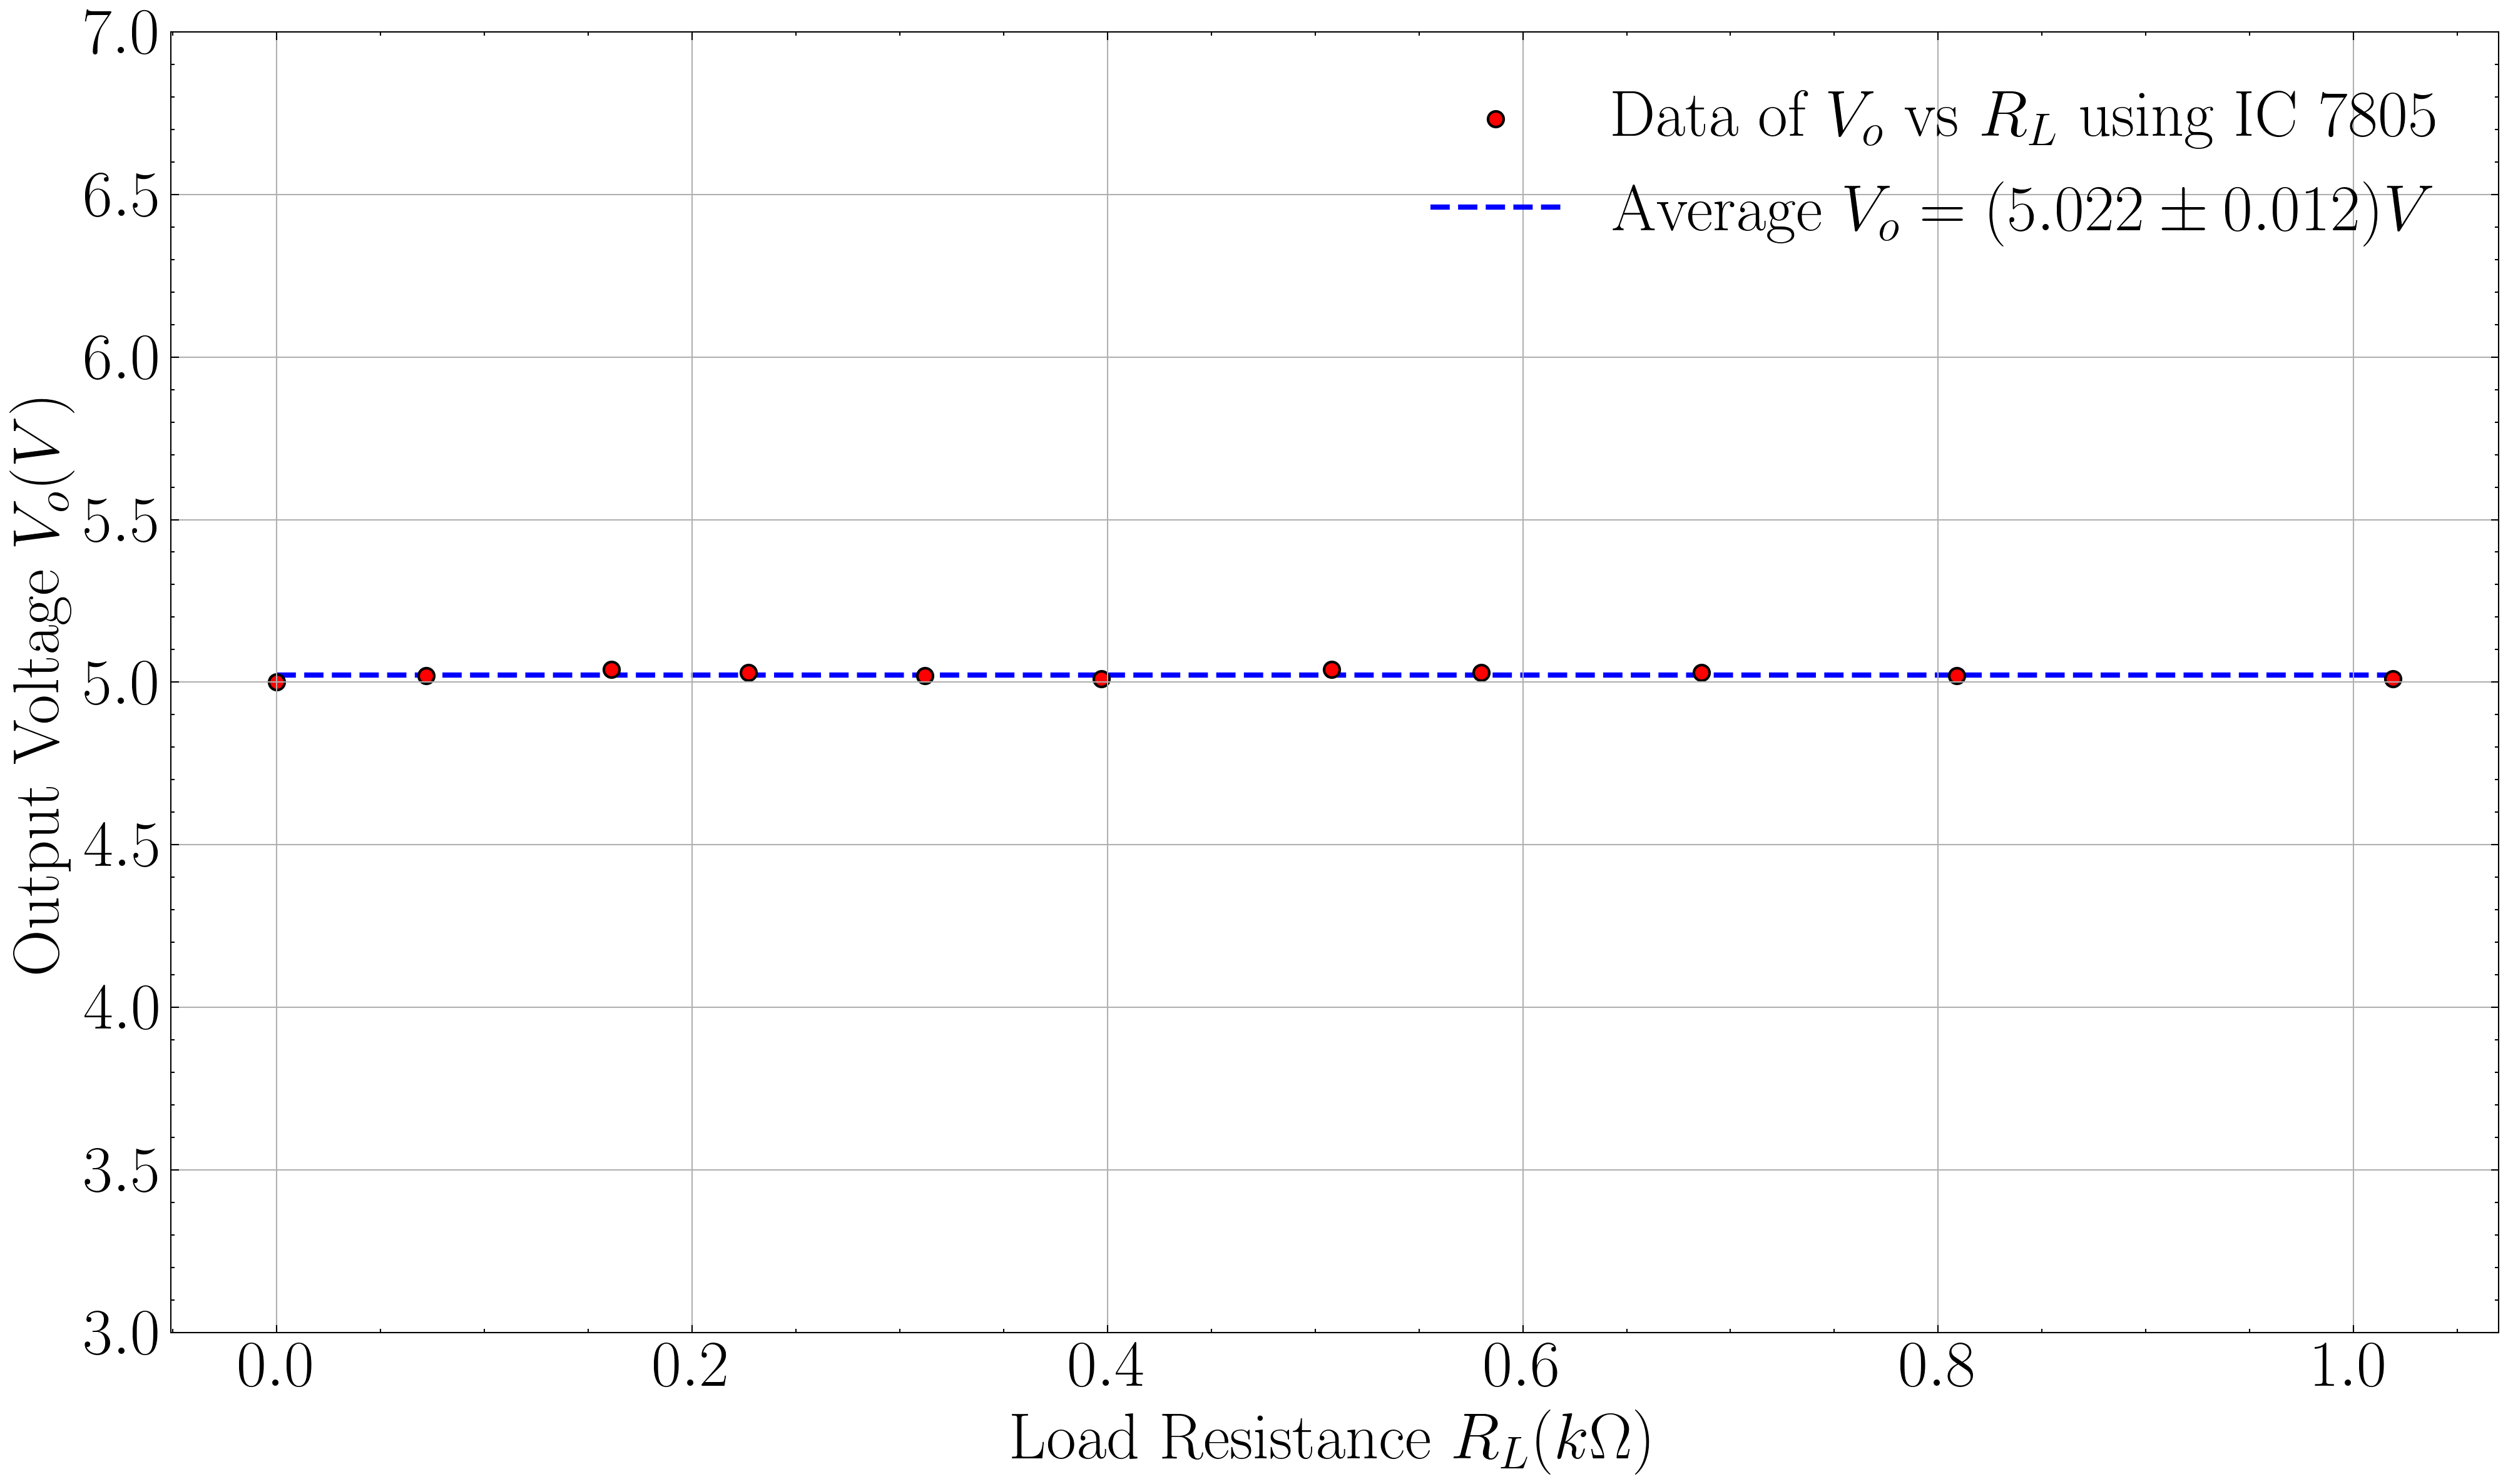
\includegraphics[width=0.8\textwidth]{icloadreg_vo_rl.png}
	\caption{$V_o$ vs $R_L$ plot for IC 7805 Load Regulation}
\end{figure}
\section{Results}
We found out from this line regulation experiment with the Zener Diode that the \textbf{breakdown voltage} is $\vb{V_b = 4.34V}$ when
the input voltage is a minimum of $\vb{V_{min} = 10.51V}$. 

On Day 2, The breakdown voltage for the load regulation experiment with $R_c = 1k\Omega$ is $\vb{V_b = 6.9V}$.

For the line and load regulation with IC 7805, the \textbf{regulated voltage} is $\vb{V_R = 5.11V}$, which 
requires a minimum input voltage of $\vb{V_{clamp} = 6.48V}$.
\section{Sources of Error}
\begin{itemize}
	\item The multimeters have limited resolution.
	\item There are fluctuations in the experiment due to errors in the DC Voltage Source.
	\item The multimeters might have internal resistances not taken into account
\end{itemize}
\section{Conclusion}
We conclude the experiment by obtaining line and load regulation using the Zener Diode and then using the more
efficient IC 7805.
\newpage
\section{Supplementary}
This is a list of the tables that were obtained during the experiment.
\begin{itemize}
	\item \textbf{Table 1}: Zener Diode Line Regulation with $R_L = 0 k\Omega$
	\item \textbf{Table 2}: Zener Load Regulation with $R_c = 2.2 k\Omega$
	\item \textbf{Table 3}: Zener Diode Load Regulation with $R_c = 1 k\Omega$
	\item \textbf{Table 4}: IC 7805 Line Regulation
	\item \textbf{Table 5}: IC 7805 Load Regulation
\end{itemize}
\begin{table}[!ht]
    \centering
    \begin{tabular}{|r|l|l|l|}
    \hline
         \textbf{$\pmb{V_i}$ (V)} & \textbf{$\pmb{I_s}$ (mA)} & \textbf{$\pmb{I_z}$ (mA)} 
		& \textbf{$\pmb{V_0}$ (V)} \\ \hline
         0 & 0 & 0 & 0 \\ \hline
         0.5 & 0.094 & 0 & 0.298 \\ \hline
         1 & 0.187 & 0 & 0.592 \\ \hline
         1.49 & 0.279 & 0 & 0.88 \\ \hline
         1.99 & 0.373 & 0 & 1.177 \\ \hline
         2.5 & 0.469 & 0 & 1.473 \\ \hline
         2.99 & 0.559 & 0 & 1.76 \\ \hline
         3.5 & 0.653 & 0.001 & 2.06 \\ \hline
         3.9 & 0.749 & 0.003 & 2.35 \\ \hline
         4.51 & 0.848 & 0.007 & 2.65 \\ \hline
         5.04 & 0.953 & 0.021 & 2.93 \\ \hline
         5.52 & 1.058 & 0.048 & 3.18 \\ \hline
         5.99 & 1.174 & 0.095 & 3.39 \\ \hline
         6.48 & 1.307 & 0.164 & 3.58 \\ \hline
         7.01 & 1.464 & 0.263 & 3.75 \\ \hline
         7.5 & 1.622 & 0.375 & 3.88 \\ \hline
         7.99 & 1.79 & 0.501 & 3.98 \\ \hline
         8.48 & 1.966 & 0.643 & 4.07 \\ \hline
         8.99 & 2.21 & 0.868 & 4.18 \\ \hline
         9.49 & 2.4 & 1.038 & 4.24 \\ \hline
         10 & 2.61 & 1.218 & 4.29 \\ \hline
         10.51 & 2.81 & 1.403 & 4.34 \\ \hline
         11.02 & 3.02 & 1.595 & 4.39 \\ \hline
         11.51 & 3.22 & 1.784 & 4.42 \\ \hline
         12.01 & 3.43 & 1.972 & 4.45 \\ \hline
         12.5 & 3.63 & 2.39 & 4.48 \\ \hline
         12.98 & 3.93 & 2.59 & 4.53 \\ \hline
         13.52 & 4.17 & 2.82 & 4.55 \\ \hline
         14.02 & 4.39 & 3.05 & 4.58 \\ \hline
         14.51 & 4.6 & 3.27 & 4.6 \\ \hline
         15 & 4.84 & 3.5 & 4.61 \\ \hline
    \end{tabular}
    \caption{Zener Diode Line Regulation with $R_L = 0 k\Omega$}
	\label{tab:ZD linereg}
\end{table} 

\begin{table}[!htb]
    \begin{minipage}{.45\linewidth}
		\centering
			\begin{tabular}{|l|l|l|l|}
			\hline
				\textbf{$\pmb{R_L(k\Omega)}$} & \textbf{$\pmb{I_L}$(mA)} & 
				\textbf{$\pmb{I_Z}$(mA)} & \textbf{$\pmb{V_o}$(V)} \\ \hline
				0 & 2.1 & 2.89 & 4.56 \\ \hline
				0.034 & 2.08 & 2.93 & 4.56 \\ \hline
				0.071 & 2.05 & 2.95 & 4.57 \\ \hline
				0.106 & 2.02 & 3.01 & 4.57 \\ \hline
				0.126 & 2 & 3.02 & 4.58 \\ \hline
				0.17 & 1.96 & 3.06 & 4.58 \\ \hline
				0.195 & 1.94 & 3.08 & 4.58 \\ \hline
				0.232 & 1.91 & 3.11 & 4.58 \\ \hline
				0.274 & 1.88 & 3.13 & 4.59 \\ \hline
				0.305 & 1.86 & 3.15 & 4.59 \\ \hline
				0.323 & 1.84 & 3.17 & 4.59 \\ \hline
				0.359 & 1.82 & 3.19 & 4.59 \\ \hline
				0.387 & 1.8 & 3.22 & 4.59 \\ \hline
				0.435 & 1.77 & 3.24 & 4.59 \\ \hline
				0.473 & 1.72 & 3.33 & 4.6 \\ \hline
				0.561 & 1.69 & 3.3 & 4.6 \\ \hline
				0.633 & 1.65 & 3.34 & 4.6 \\ \hline
				0.721 & 1.6 & 3.37 & 4.6 \\ \hline
				0.826 & 1.55 & 3.44 & 4.61 \\ \hline
				0.919 & 1.48 & 3.53 & 4.62 \\ \hline
				1.025 & 1.45 & 3.53 & 4.62 \\ \hline
			\end{tabular}
			\caption{Zener Load Reg. with $R_c = 2.2 k\Omega$}
			\label{tab:ZDload2.2ohm}
    \end{minipage}%
    \begin{minipage}{.5\linewidth}
      \centering
    \begin{tabular}{|l|l|l|l|}
    \hline
        \textbf{$\pmb{R_L(k\Omega)}$} & \textbf{$\pmb{I_L}$(mA)} 
		& \textbf{$\pmb{I_Z}$(mA)} & \textbf{$\pmb{V_o}$(V)} \\ \hline
        1.45 & 4.15 & 0 & 6.03 \\ \hline
        1.473 & 4.13 & 0 & 6.07 \\ \hline
        1.486 & 4.12 & 0 & 6.1 \\ \hline
        1.492 & 4.11 & 0 & 6.12 \\ \hline
        1.497 & 4.1 & 0 & 6.14 \\ \hline
        1.521 & 4.09 & 0 & 6.16 \\ \hline
        1.528 & 4.07 & 0.01 & 6.18 \\ \hline
        1.584 & 4.06 & 0.02 & 6.22 \\ \hline
        1.563 & 4.03 & 0.02 & 6.26 \\ \hline
        1.583 & 3.98 & 0.04 & 6.34 \\ \hline
        1.626 & 3.96 & 0.05 & 6.35 \\ \hline
        1.616 & 3.95 & 0.06 & 6.36 \\ \hline
        1.661 & 3.88 & 0.1 & 6.41 \\ \hline
        1.967 & 3.29 & 0.67 & 6.44 \\ \hline
        2.04 & 3.16 & 0.8 & 6.46 \\ \hline
    \end{tabular}
    \caption{Zener Diode Load Regulation with $R_c = 1 k\Omega$}
	\label{tab:ZDload1ohm}
    \end{minipage} 
\end{table}






\begin{table}[!htb]
	\centering
    \begin{minipage}{.35\linewidth}
		\centering
    \begin{tabular}{|l|l|l|}
    \hline
        $\pmb{V_i (V)}$ & $\pmb{I_L (mA)}$ & $\pmb{V_o (V)}$ \\ \hline
        0.1 & 0 & 0 \\ \hline
        0.52 & 0 & 0 \\ \hline
        1 & 0 & 0.0001 \\ \hline
        1.5 & 0.02 & 0.05 \\ \hline
        2.06 & 0.63 & 1.299 \\ \hline
        2.49 & 0.81 & 1.697 \\ \hline
        3.02 & 1.04 & 2.19 \\ \hline
        3.45 & 1.23 & 2.61 \\ \hline
        4.03 & 1.47 & 3.1 \\ \hline
        4.5 & 1.67 & 3.53 \\ \hline
        5.04 & 1.9 & 4.03 \\ \hline
        5.54 & 2.12 & 4.49 \\ \hline
        6.03 & 2.33 & 4.94 \\ \hline
        6.48 & 2.42 & 5.12 \\ \hline
        6.95 & 2.42 & 5.11 \\ \hline
        7.47 & 2.42 & 5.11 \\ \hline
        8 & 2.41 & 5.11 \\ \hline
        8.52 & 2.43 & 5.11 \\ \hline
        9.01 & 2.43 & 5.11 \\ \hline
    \end{tabular}
    \caption{IC 7805 Line Regulation}
	\label{tab:icline}
    \end{minipage}%
    \begin{minipage}{.45\linewidth}
		\centering
    \begin{tabular}{|l|l|l|l|}
    \hline
        $\pmb{R_L (k \Omega)}$ & $\pmb{V_i (V)}$ & $\pmb{I_L (mA)}$ & $\pmb{V_o (V)}$ \\ \hline
        0 & 15 & 2.35 & 5 \\ \hline
        0.072 & 15 & 2.3 & 5.02 \\ \hline
        0.161 & 15 & 2.21 & 5.04 \\ \hline
        0.227 & 15 & 2.15 & 5.03 \\ \hline
        0.312 & 15 & 2.08 & 5.02 \\ \hline
        0.397 & 15 & 2 & 5.01 \\ \hline
        0.508 & 15 & 1.93 & 5.04 \\ \hline
        0.58 & 15 & 1.87 & 5.03 \\ \hline
        0.686 & 15 & 1.78 & 5.03 \\ \hline
        0.809 & 15 & 1.71 & 5.02 \\ \hline
        1.019 & 15 & 1.61 & 5.01 \\ \hline
    \end{tabular}
    \caption{IC 7805 Load Regulation}
	\label{tab:icload}
    \end{minipage} 
\end{table}

% lol tables

% \begin{table}[!ht]
%     \centering
%     \begin{tabular}{|l|l|l|l|}
%     \hline
%         \textbf{R\_L(kO)} & \textbf{i\_L(mA)} & \textbf{i\_Z(mA)} & \textbf{V\_o(V)} \\ \hline
%         0 & 2.1 & 2.89 & 4.56 \\ \hline
%         0.034 & 2.08 & 2.93 & 4.56 \\ \hline
%         0.071 & 2.05 & 2.95 & 4.57 \\ \hline
%         0.106 & 2.02 & 3.01 & 4.57 \\ \hline
%         0.126 & 2 & 3.02 & 4.58 \\ \hline
%         0.17 & 1.96 & 3.06 & 4.58 \\ \hline
%         0.195 & 1.94 & 3.08 & 4.58 \\ \hline
%         0.232 & 1.91 & 3.11 & 4.58 \\ \hline
%         0.274 & 1.88 & 3.13 & 4.59 \\ \hline
%         0.305 & 1.86 & 3.15 & 4.59 \\ \hline
%         0.323 & 1.84 & 3.17 & 4.59 \\ \hline
%         0.359 & 1.82 & 3.19 & 4.59 \\ \hline
%         0.387 & 1.8 & 3.22 & 4.59 \\ \hline
%         0.435 & 1.77 & 3.24 & 4.59 \\ \hline
%         0.473 & 1.72 & 3.33 & 4.6 \\ \hline
%         0.561 & 1.69 & 3.3 & 4.6 \\ \hline
%         0.633 & 1.65 & 3.34 & 4.6 \\ \hline
%         0.721 & 1.6 & 3.37 & 4.6 \\ \hline
%         0.826 & 1.55 & 3.44 & 4.61 \\ \hline
%         0.919 & 1.48 & 3.53 & 4.62 \\ \hline
%         1.025 & 1.45 & 3.53 & 4.62 \\ \hline
%     \end{tabular}
%     \caption{Zener Diode Load Regulation with $R_c = 2.2 k\Omega$}
% \end{table}
% \begin{table}[!ht]
%     \centering
%     \begin{tabular}{|l|l|l|l|}
%     \hline
%         \textbf{R\_L(kO)} & \textbf{i\_L(mA)} & \textbf{i\_Z(mA)} & \textbf{V\_o(V)} \\ \hline
%         1.45 & 4.15 & 0 & 6.03 \\ \hline
%         1.473 & 4.13 & 0 & 6.07 \\ \hline
%         1.486 & 4.12 & 0 & 6.1 \\ \hline
%         1.492 & 4.11 & 0 & 6.12 \\ \hline
%         1.497 & 4.1 & 0 & 6.14 \\ \hline
%         1.521 & 4.09 & 0 & 6.16 \\ \hline
%         1.528 & 4.07 & 0.01 & 6.18 \\ \hline
%         1.584 & 4.06 & 0.02 & 6.22 \\ \hline
%         1.563 & 4.03 & 0.02 & 6.26 \\ \hline
%         1.583 & 3.98 & 0.04 & 6.34 \\ \hline
%         1.626 & 3.96 & 0.05 & 6.35 \\ \hline
%         1.616 & 3.95 & 0.06 & 6.36 \\ \hline
%         1.661 & 3.88 & 0.1 & 6.41 \\ \hline
%         1.967 & 3.29 & 0.67 & 6.44 \\ \hline
%         2.04 & 3.16 & 0.8 & 6.46 \\ \hline
%     \end{tabular}
%     \caption{Zener Diode Load Regulation with $R_c = 1 k\Omega$}
% \end{table}

% \begin{table}[!ht]
%     \centering
%     \begin{tabular}{|l|l|l|}
%     \hline
%         Vi (Volts) & iL (mA) & V0 (V) \\ \hline
%         0.1 & 0 & 0 \\ \hline
%         0.52 & 0 & 0 \\ \hline
%         1 & 0 & 0.0001 \\ \hline
%         1.5 & 0.02 & 0.05 \\ \hline
%         2.06 & 0.63 & 1.299 \\ \hline
%         2.49 & 0.81 & 1.697 \\ \hline
%         3.02 & 1.04 & 2.19 \\ \hline
%         3.45 & 1.23 & 2.61 \\ \hline
%         4.03 & 1.47 & 3.1 \\ \hline
%         4.5 & 1.67 & 3.53 \\ \hline
%         5.04 & 1.9 & 4.03 \\ \hline
%         5.54 & 2.12 & 4.49 \\ \hline
%         6.03 & 2.33 & 4.94 \\ \hline
%         6.48 & 2.42 & 5.12 \\ \hline
%         6.95 & 2.42 & 5.11 \\ \hline
%         7.47 & 2.42 & 5.11 \\ \hline
%         8 & 2.41 & 5.11 \\ \hline
%         8.52 & 2.43 & 5.11 \\ \hline
%         9.01 & 2.43 & 5.11 \\ \hline
%     \end{tabular}
%     \caption{IC 7805 Line Regulation}
% \end{table}
% \begin{table}[!ht]
%     \centering
%     \begin{tabular}{|l|l|l|l|}
%     \hline
%         RL (k ohms) & Vi (Volts) & iL (mA) & V0 (V) \\ \hline
%         0 & 15 & 2.35 & 5 \\ \hline
%         0.072 & 15 & 2.3 & 5.02 \\ \hline
%         0.161 & 15 & 2.21 & 5.04 \\ \hline
%         0.227 & 15 & 2.15 & 5.03 \\ \hline
%         0.312 & 15 & 2.08 & 5.02 \\ \hline
%         0.397 & 15 & 2 & 5.01 \\ \hline
%         0.508 & 15 & 1.93 & 5.04 \\ \hline
%         0.58 & 15 & 1.87 & 5.03 \\ \hline
%         0.686 & 15 & 1.78 & 5.03 \\ \hline
%         0.809 & 15 & 1.71 & 5.02 \\ \hline
%         1.019 & 15 & 1.61 & 5.01 \\ \hline
%     \end{tabular}
%     \caption{IC 7805 Load Regulation}
% \end{table}
\end{document}
